\documentclass{beamer}

% --- Tema ---
\usetheme{SimpleDarkBlue}

\usepackage{hyperref}
\usepackage{graphicx} 
\usepackage{booktabs} 
\usepackage{tikz}
\usepackage{verbatim}

% --- Metadados ---
\title{ICP133 -  Fundamentos de Sistemas de Computação}
\author{Prof. Gabriel Rodrigues Caldas de Aquino}

\institute
{
    Instituto de Computação \\
    Universidade Federal do Rio de Janeiro\\
    gabrielaquino@ic.ufrj.br
}
\date{Compilado em: \\ \today} 

\begin{document}

\begin{frame}
    \titlepage
\end{frame}

%\title{Aula 1 - Apresentação do curso}



\begin{frame}
    \titlepage
\end{frame}

\begin{frame}{Literatura}
    \centering
    \begin{columns}
        \begin{column}{0.5\linewidth}
            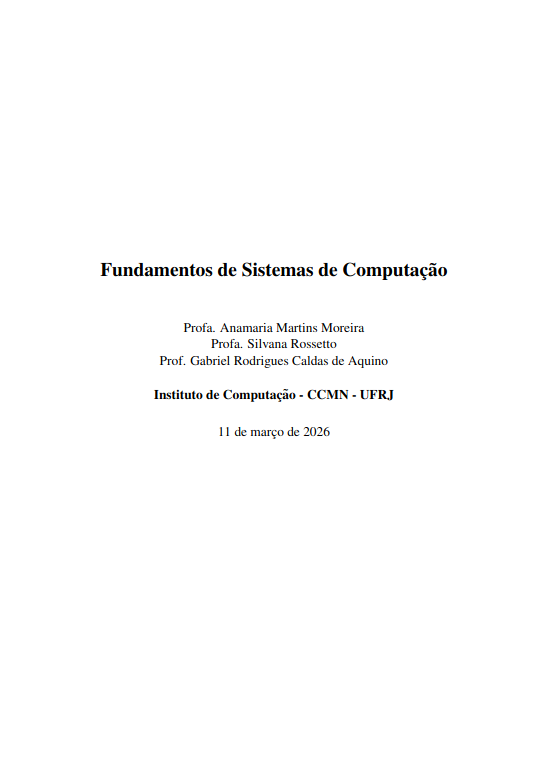
\includegraphics[width=0.8\linewidth]{Figuras/apostfund.png}
        \end{column}
        \begin{column}{0.5\linewidth}
            \begin{itemize}
                \item Apostila de fundamentos
                \item \href{URL}{Baixe a apostila}
            \end{itemize}
        \end{column}
    \end{columns}

\end{frame}

\begin{frame}{Literatura}
    \centering
    \begin{columns}
        \begin{column}{0.5\linewidth}
            \begin{itemize}
                \item Sistemas digitais: princípios e aplicações \\ Ronald J.
                      Tocci, Neal S. Widmer, Gregory L. Moss; \\ tradução
                      Jorge Ritter; revisão técnica Renato Giacomini. – 11. ed.
                      – São Paulo: Pearson Prentice Hall, 2011.
                      \\Título original: Digital systems: principles and applications
                      \\ISBN 978-85-430-0694-9
            \end{itemize}
        \end{column}
        \begin{column}{0.5\linewidth}
            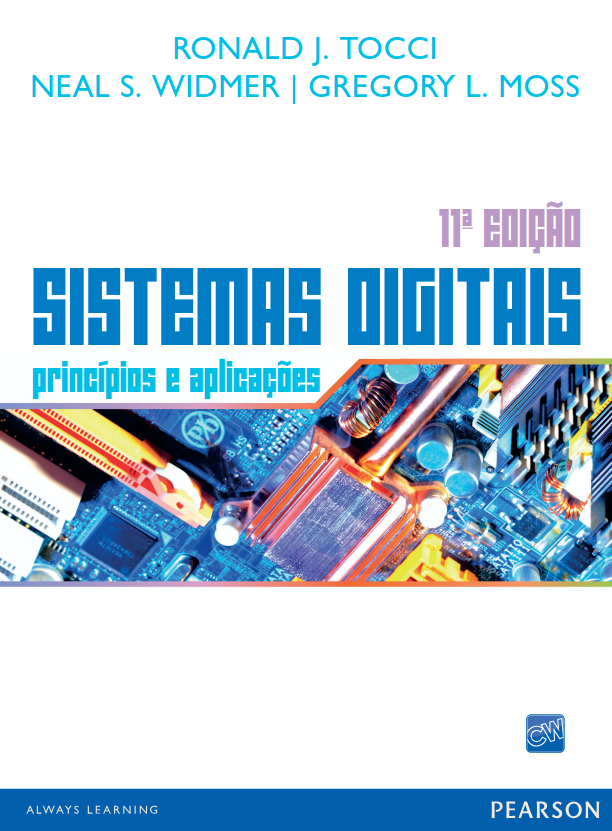
\includegraphics[width=0.8\linewidth]{Figuras/livro-sistdig.png}
        \end{column}
    \end{columns}

\end{frame}


\begin{frame}{Método de Avaliação}
    \textbf{Componentes da Nota}
    \begin{itemize}
        \item \textbf{Provas (P1, P2 e P3):}
              Média das provas (MP) $\rightarrow$ 80\% da nota

    \end{itemize}


    \textbf{Critério de Aprovação Direta}
    \begin{itemize}
        \item Média ponderada de das provas (P1, P2 e P3) $\geq 7$
              \hspace{1em} $\rightarrow$ Aprovado direto
        \item Se $3 <= \text{Média ponderada } <= 7$
              \hspace{1em} $\rightarrow$ Prova final (PF)
    \end{itemize}


    \textbf{Cálculo da Média Final}
    \[
        \text{Média final} = \frac{\text{Média anterior} + \text{PF}}{2}
    \]
    \begin{itemize}
        \item Se $\text{Média final} \geq 5$ $\Rightarrow$ Aprovado
        \item Caso contrário $\Rightarrow$ Reprovado
    \end{itemize}


\end{frame}



\begin{frame}{O Sistema do Telégrafo}
    \begin{itemize}
        \item \textbf{Funcionamento Eletromecânico:}
              \begin{itemize}
                  \item Circuito composto por bateria, chave (transmissor) e bobina (receptor).
                  \item O fechamento da chave cria um campo magnético que atrai uma placa metálica ("estalido").
                  \item O retorno por mola ao abrir o circuito gera um som distinto.
              \end{itemize}
        \item \textbf{Representação Digital:}
              \begin{itemize}
                  \item Uso de dois símbolos distintos: \textbf{pontos} (pulsos curtos) e \textbf{traços} (pulsos longos).
                  \item Base do Código Morse: a informação é codificada na \textbf{duração} e na \textbf{sequência} dos pulsos.
              \end{itemize}
    \end{itemize}

\end{frame}

\begin{frame}{Diagramas de Tempos e Sinais}
    \begin{center}
        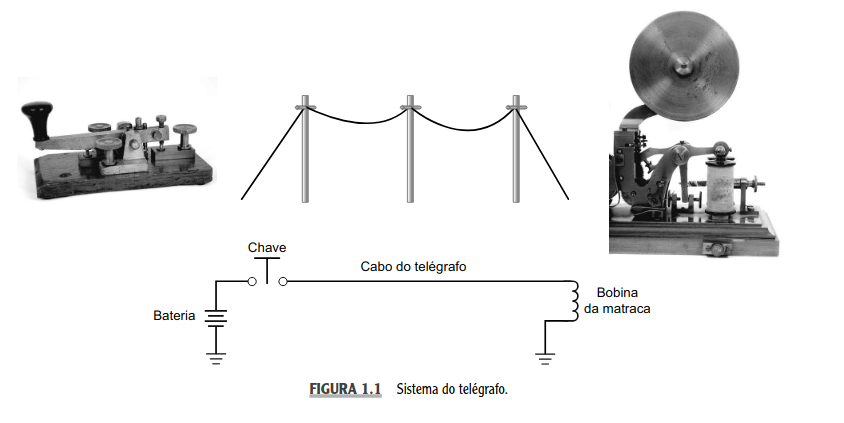
\includegraphics[width=0.8\textwidth]{Figuras/telegrafo.png}

    \end{center}
    \begin{itemize}
        \item \textbf{Natureza do Sinal:}
              \begin{itemize}
                  \item O sinal elétrico é binário: está sempre \textbf{ligado} ou \textbf{desligado}.
                  \item Precursor dos sistemas modernos (níveis lógicos 0 e 1).
              \end{itemize}
        \item \textbf{Diagrama de Tempos:}
              \begin{itemize}
                  \item Gráfico da tensão (ou corrente) versus tempo ($x = t$).
                  \item \textbf{Função:} Mostra o estado do sistema em qualquer instante e o momento exato das transições.
              \end{itemize}
    \end{itemize}





\end{frame}


\begin{frame}[t]{Diagramas de Tempo}
    \begin{itemize}
        \item Representação gráfica da atividade em sistemas digitais
        \item Eixo \textbf{x}: tempo
        \item Eixo \textbf{y}: estado (1 ou 0)
        \item Mostra:
              \begin{itemize}
                  \item Estado do sistema em qualquer momento
                  \item Momento exato das mudanças de estado
              \end{itemize}
        \item \textbf{Ferramenta fundamental} para análise de sistemas digitais
    \end{itemize}

    \begin{center}
        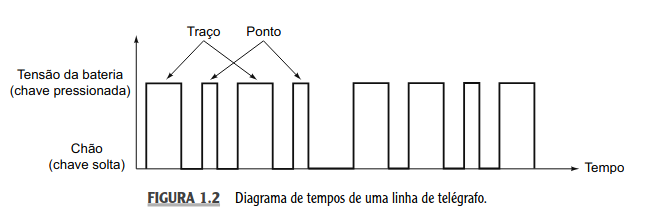
\includegraphics[width=0.9\textwidth]{Figuras/diagrama-de-tempo.png}

    \end{center}
\end{frame}

\begin{frame}{Representação Analógica}
    \begin{itemize}
        \item \textbf{Definição:} Uma quantidade é representada por um indicador proporcional \textbf{continuamente variável}.
        \item \textbf{Características Principais:}
              \begin{itemize}
                  \item Acompanha variações mínimas de forma fluida.
                  \item O indicador (ponteiro, coluna, tensão) "segue" a grandeza física.
              \end{itemize}
        \item \textbf{Exemplos Clássicos:}
              \begin{itemize}
                  \item \textbf{Velocímetro Mecânico:} Deflexão do ponteiro proporcional à velocidade do eixo.
                  \item \textbf{Termômetro de Mercúrio:} Altura da coluna varia com a temperatura.
                  \item \textbf{Termômetro de Mola:} Expansão/contração térmica converte-se em posição angular.
              \end{itemize}
    \end{itemize}
\end{frame}

\begin{frame}{Sistemas Analógicos Elétricos}
    \begin{itemize}
        \item \textbf{Conversão de Grandezas:}
              \begin{itemize}
                  \item A quantidade física original é convertida em um \textbf{sinal elétrico}.
                  \item A \textbf{tensão} ou \textbf{corrente} resultante é diretamente proporcional à medida.
              \end{itemize}
        \item \textbf{Aplicações:}
              \begin{itemize}
                  \item Exibição em escalas graduadas.
                  \item Processamento de sinais em tempo real.
                  \item Sistemas de controle contínuo.
              \end{itemize}
    \end{itemize}
    \vspace{0.3cm}

\end{frame}

\begin{frame}{O Som como Grandeza Analógica}
    \begin{itemize}
        \item \textbf{Histórico:} Alexander Graham Bell (1875) converteu voz em sinal elétrico continuamente variável.
        \item \textbf{O Microfone:} Atua como um transdutor que converte energia sonora em \textbf{tensão analógica}.
        \item \textbf{Características do Sinal de Voz:}
              \begin{itemize}
                  \item \textbf{Frequência ($f$):} Ciclos por segundo; define os tons da voz.
                  \item \textbf{Período ($T$):} Tempo de cada ciclo ($T = 1/f$).
                  \item \textbf{Amplitude:} Medida no eixo vertical (Volts); define a \textbf{intensidade} (volume) e a inflexão da fala.
              \end{itemize}
    \end{itemize}

\end{frame}

\begin{frame}{Onda de Audio}
    \begin{center}
        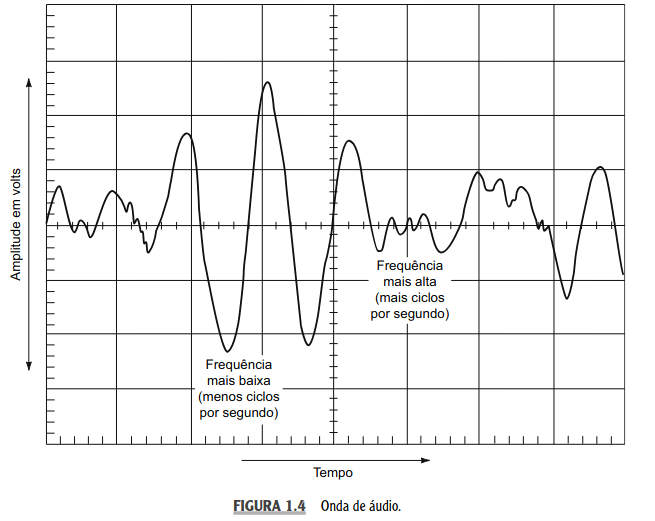
\includegraphics[width=0.7\textwidth]{Figuras/onda-de-audio.png}

    \end{center}


\end{frame}

\begin{frame}{A Natureza Contínua das Quantidades}
    \begin{itemize}
        \item \textbf{Característica Fundamental:} Variam ao longo de uma \textbf{faixa contínua} de valores.
        \item \textbf{Exemplos de Faixas Típicas:}
    \end{itemize}
    \begin{table}[]
        \centering
        \begin{tabular}{|l|l|}
            \hline
            \textbf{Grandeza}  & \textbf{Exemplo de Faixa} \\ \hline
            Velocidade         & 0 a 160 km/h              \\ \hline
            Temperatura        & -29°C a 49°C              \\ \hline
            Tensão (Microfone) & 0 a $V_{max}$             \\ \hline
        \end{tabular}
    \end{table}
    \begin{block}{Conclusão}
        Diferente do digital (degraus), o analógico não possui "saltos"; entre dois valores quaisquer, existe uma infinidade de valores intermediários.
    \end{block}
\end{frame}

\begin{frame}{Representação Digital}
    \begin{itemize}
        \item \textbf{Definição:} Quantidades representadas por símbolos chamados \textbf{dígitos}, em vez de indicadores contínuos.
        \item \textbf{Funcionamento:}
              \begin{itemize}
                  \item A variação ocorre em \textbf{incrementos discretos} (saltos).
                  \item Exemplo: Um termômetro digital que mede de $0,1^{\circ}\text{C}$ em $0,1^{\circ}\text{C}$.
                  \item A temperatura real sobe de forma fluida, mas o visor "pula" de $22,0^{\circ}\text{C}$ para $22,1^{\circ}\text{C}$.
              \end{itemize}
    \end{itemize}
    \vspace{0.3cm}
    \begin{center}
        \begin{tabular}{|c|c|}
            \hline
            \textbf{Analógica}    & \textbf{Digital}          \\ \hline
            Contínua              & Discreta (Passo a passo)  \\ \hline
            Infinidade de valores & Valores finitos/definidos \\ \hline
        \end{tabular}
    \end{center}
\end{frame}

\begin{frame}{Analógico vs. Digital}
    \begin{itemize}
        \item \textbf{Comparação Visual:}
              \begin{itemize}
                  \item O analógico é como uma \textbf{rampa} (suave).
                  \item O digital é como uma \textbf{escada} (degraus).
              \end{itemize}
        \item \textbf{Precisão e Resolução:}
              \begin{itemize}
                  \item No digital, a precisão depende do número de dígitos ou "passos" disponíveis no sistema.
              \end{itemize}
    \end{itemize}

    \begin{block}{Diferença Fundamental}
        \centering
        \textbf{Analógica $\equiv$ Contínua} \\
        \textbf{Digital $\equiv$ Discreta}
    \end{block}
\end{frame}

\begin{frame}{Ambiguidade vs. Precisão Digital}
    \begin{itemize}
        \item \textbf{Interpretação Analógica:}
              \begin{itemize}
                  \item Frequentemente sujeita a interpretação livre (ex: posição exata de um ponteiro entre dois traços).
                  \item Depende da percepção do observador.
              \end{itemize}
        \item \textbf{Ausência de Ambiguidade Digital:}
              \begin{itemize}
                  \item A leitura é direta e numérica.
                  \item Não há dúvida sobre o valor exibido (ex: $22,5^{\circ}\text{C}$ é lido exatamente como tal).
              \end{itemize}
        \item \textbf{O Processo de Digitalização:}
              \begin{itemize}
                  \item Na prática, sempre "arredondamos" medidas analógicas para um nível de precisão conveniente.
                  \item \textbf{Digitalizar:} Atribuir um número de \textbf{precisão limitada} a uma quantidade continuamente variável.
              \end{itemize}
    \end{itemize}
\end{frame}

\begin{frame}{Utilidade das Representações Digitais}
    \begin{itemize}
        \item \textbf{Captura do Mundo Real:}
              \begin{itemize}
                  \item O mundo é analógico (variáveis mudam constantemente).
                  \item Ao medir e converter essas variáveis em quantidades digitais, ganhamos novas possibilidades.
              \end{itemize}
        \item \textbf{Vantagens do Processamento Digital:}
              \begin{itemize}
                  \item \textbf{Registro:} Armazenamento fiel de dados ao longo do tempo.
                  \item \textbf{Manipulação:} Cálculos aritméticos e algoritmos complexos.
                  \item \textbf{Controle:} Uso das informações para acionar ou gerenciar sistemas.
              \end{itemize}
    \end{itemize}

\end{frame}

\begin{frame}{Quiz - Analógico ou digital?}
    \begin{center}
        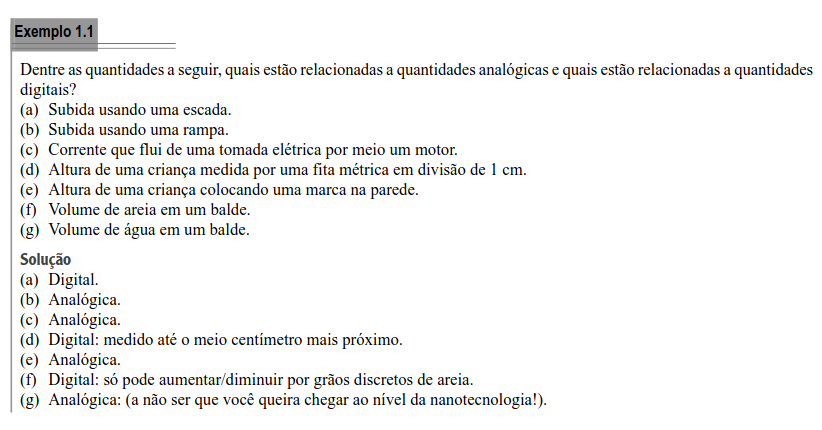
\includegraphics[width=\textwidth]{Figuras/quiz-analogico-digital.png}

    \end{center}


\end{frame}

\begin{frame}{Definição de Sistemas}
    \begin{itemize}
        \item \textbf{Sistemas Digitais:}
              \begin{itemize}
                  \item Combinação de dispositivos para manipular informação lógica ou quantidades em \textbf{valores discretos}.
                  \item \textbf{Meios:} Eletrônicos (mais comuns), mecânicos, magnéticos ou pneumáticos.
                  \item \textbf{Exemplos:} Computadores, calculadoras, sistemas de telecomunicações.
              \end{itemize}
        \item \textbf{Sistemas Analógicos:}
              \begin{itemize}
                  \item Dispositivos que manipulam quantidades em \textbf{faixas contínuas}.
                  \item \textbf{Exemplo:} O sinal de saída de um alto-falante (pode assumir qualquer amplitude entre zero e o máximo).
              \end{itemize}
    \end{itemize}
\end{frame}

\begin{frame}{Sistemas de Sinal Híbrido ou Misto}
    \begin{itemize}
        \item \textbf{Integração:} É comum o uso de ambas as técnicas em um mesmo projeto para aproveitar as vantagens específicas de cada uma.
        \item \textbf{Desafio de Projeto:} Determinar quais partes do fluxo devem ser analógicas e quais devem ser digitais.
        \item \textbf{Tendência Atual:}
              \begin{enumerate}
                  \item Digitalizar o sinal \textbf{o mais cedo possível}.
                  \item Processar digitalmente.
                  \item Converter de volta para analógico \textbf{o mais tarde possível}.
              \end{enumerate}
    \end{itemize}




    A digitalização precoce preserva a integridade da informação contra ruídos e facilita o processamento complexo.

\end{frame}

\begin{frame}{Evolução do Telefone: Um Sistema Híbrido}
    \begin{itemize}
        \item \textbf{A Visão de Bell:} Para utilidade real, os telefones precisavam funcionar em \textbf{rede}.
        \item \textbf{Sinalização (Digital):}
              \begin{itemize}
                  \item Gerador a manivela produzia tensão para as campainhas.
                  \item Cada usuário possuía um \textbf{código único} de toques (curtos e longos).
                  \item \textbf{Codificação:} Feita manualmente pelo emissor ao girar a manivela.
                  \item \textbf{Decodificação:} Feita mentalmente pelo receptor ao ouvir o padrão.
              \end{itemize}
        \item \textbf{Comunicação (Analógica):}
              \begin{itemize}
                  \item Uma vez estabelecida a conexão, a voz era transmitida de forma puramente analógica.
              \end{itemize}
    \end{itemize}
    \emph{Conceito Histórico}:
    O sistema de telefonia inicial já utilizava o conceito de \textbf{sinalização digital} para endereçamento e \textbf{transmissão analógica} para o conteúdo.

\end{frame}

\begin{frame}{Evolução: Telefones de Disco e Teclas}
    \begin{itemize}
        \item \textbf{Telefone de Disco (Pulsos):}
              \begin{itemize}
                  \item Sistema de numeração decimal representado por séries de pulsos.
                  \item \textbf{Mecanismo:} A mola de retorno girava um eixo de came que abria/fechava contatos.
                  \item \textbf{Exemplo:} 9 pulsos = número 9; 10 pulsos = número 0.
                  \item \textbf{Decodificação:} Máquinas eletromecânicas interpretavam os pulsos para realizar a conexão automática.
              \end{itemize}
        \item \textbf{Telefone de Teclas (DTMF):}
              \begin{itemize}
                  \item \textbf{DTMF:} \textit{Dual Tone Multiple Frequency}.
                  \item Cada dígito é representado por um sinal audível composto pela combinação de \textbf{duas frequências senoidais}.
                  \item Circuitos eletrônicos reconhecem os tons e os traduzem em sequência digital.
              \end{itemize}
    \end{itemize}
    \begin{block}{Integração}
        A informação digital (números) é enviada via sinais analógicos (tons), demonstrando a coexistência histórica das duas tecnologias.
    \end{block}
\end{frame}

\begin{frame}{Vantagens das Técnicas Digitais (1/2)}
    \begin{itemize}
        \item \textbf{Facilidade de Projeto:}
              \begin{itemize}
                  \item Baseado em circuitos de \textbf{chaveamento}.
                  \item Importam apenas as faixas (\textit{HIGH} ou \textit{LOW}), não valores exatos de tensão.
              \end{itemize}
        \item \textbf{Armazenamento Eficiente:}
              \begin{itemize}
                  \item Dispositivos especiais (\textit{latches}) mantêm a informação indefinidamente.
                  \item Armazenamento de massa: bilhões de bits em espaços reduzidos.
              \end{itemize}
        \item \textbf{Precisão e Exatidão:}
              \begin{itemize}
                  \item A informação não se deteriora durante o processamento.
                  \item Sistemas analógicos sofrem com variações de temperatura, umidade e tolerância de componentes.
              \end{itemize}
    \end{itemize}
\end{frame}

\begin{frame}{Vantagens das Técnicas Digitais (2/2)}
    \begin{itemize}
        \item \textbf{Operações Programáveis:}
              \begin{itemize}
                  \item Comportamento controlado por conjuntos de instruções (programas).
                  \item Flexibilidade e complexidade muito superiores aos sistemas analógicos.
              \end{itemize}
        \item \textbf{Imunidade ao Ruído:}
              \begin{itemize}
                  \item Flutuações de tensão (ruído) são desprezíveis, desde que não alterem a distinção entre nível \textbf{ALTO} e \textbf{BAIXO}.
              \end{itemize}

        \item \textbf{Alta Integração (CIs):}
              \begin{itemize}
                  \item Chips digitais comportam milhões de dispositivos.
                  \item Analógicos exigem componentes difíceis de integrar (grandes capacitores, indutores, resistores de precisão).
              \end{itemize}
    \end{itemize}
\end{frame}

\begin{frame}{Limitações das Técnicas Digitais}
    Apesar das vantagens, existem dois desafios principais na adoção do digital:
    \begin{itemize}
        \item \textbf{O Mundo Real é Analógico:}
              \begin{itemize}
                  \item Grandezas físicas (temperatura, pressão, velocidade, vazão) são contínuas por natureza.
                  \item Representações como "18°C" são apenas \textbf{aproximações digitais} da realidade.
              \end{itemize}
        \item \textbf{Tempo de Processamento:}
              \begin{itemize}
                  \item Converter, processar e desconverter sinais exige tempo (latência), o que pode ser crítico em sistemas de altíssima velocidade.
              \end{itemize}
    \end{itemize}
    \begin{exampleblock}{Exemplos de Sensores no Automóvel}
        Nível de combustível, temperatura do motor, acelerômetros (airbag) e sensores de pressão.
    \end{exampleblock}
\end{frame}

\begin{frame}{Lidando com o Mundo Analógico}
    Para integrar o processamento digital ao mundo físico, seguimos quatro passos fundamentais:
    \begin{enumerate}
        \item \textbf{Transdução:} Converter a variável física (ex: calor) em sinal elétrico analógico.
        \item \textbf{Conversão A/D:} Transformar o sinal analógico em formato digital (bits).
        \item \textbf{Processamento:} Operar a informação digitalmente (cálculos, lógica).
        \item \textbf{Conversão D/A:} Converter o resultado digital de volta para o formato analógico do mundo real.
    \end{enumerate}

\end{frame}

\begin{frame}{Estudo de Caso: Controle de Temperatura}
    \begin{itemize}
        \item \textbf{Entrada de Usuário (Digital):} Ajuste da temperatura desejada em incrementos discretos (ex: $0,1^{\circ}\text{C}$).
        \item \textbf{Captura (Analógica):} Um sensor converte a temperatura ambiente em uma \textbf{tensão proporcional}.
        \item \textbf{Interface de Processamento:}
              \begin{itemize}
                  \item \textbf{ADC (Conversor Analógico-Digital):} Traduz a tensão do sensor para um valor binário.
                  \item \textbf{Processador:} Compara o valor real com o desejado e calcula a correção necessária.
              \end{itemize}
    \end{itemize}

\end{frame}

\begin{frame}{Atuação e Ciclo de Controle}
    \begin{itemize}
        \item \textbf{Saída do Sistema:}
              \begin{itemize}
                  \item \textbf{DAC (Conversor Digital-Analógico):} Converte o ajuste digital calculado de volta para uma \textbf{tensão analógica}.
                  \item \textbf{Atuador:} O dispositivo de aquecimento recebe essa tensão e gera calor proporcional para o ambiente.
              \end{itemize}
        \item \textbf{Resumo do Fluxo:}
    \end{itemize}
    \begin{center}
        \fbox{Temp. Física} $\rightarrow$ \textbf{Sensor} $\rightarrow$ \textbf{ADC} $\rightarrow$ \textbf{Lógica Digital} $\rightarrow$ \textbf{DAC} $\rightarrow$ \textbf{Aquecedor}
    \end{center}
    \begin{block}{Importância da Conversão}
        Este ciclo permite que a precisão da lógica digital controle variáveis instáveis e contínuas do mundo físico.
    \end{block}
\end{frame}

\begin{frame}{Exemplo}
    \begin{center}
        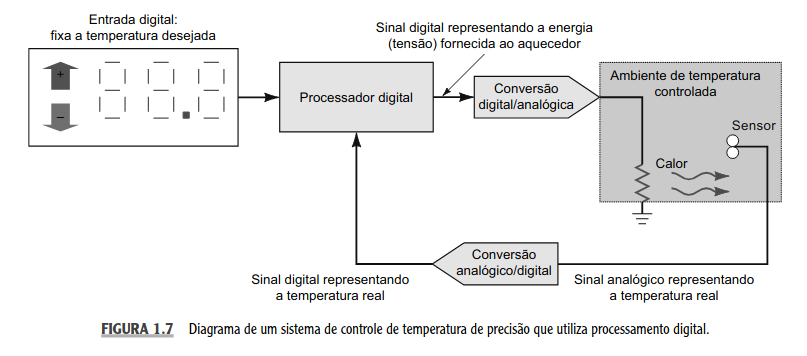
\includegraphics[width=\textwidth]{Figuras/temperatura-procdigital.png}

    \end{center}


\end{frame}

\begin{frame}{Exemplo de Transdutor: O LDR}
    \begin{itemize}
        \item \textbf{Definição:} O \textit{Light Dependent Resistor} (Resistor Dependente de Luz) é um componente analógico cuja resistência varia com a intensidade luminosa.
        \item \textbf{Comportamento Analógico:}
              \begin{itemize}
                  \item Varia a resistencia com a luz.
                  \item A variação é \textbf{contínua} e proporcional à luz recebida.
              \end{itemize}
        \item \textbf{Integração Digital:}
              \begin{itemize}
                  \item O LDR envia uma \textbf{tensão analógica} para um pino do microcontrolador.
                  \item O \textbf{ADC} interno converte essa tensão em um número.
              \end{itemize}
    \end{itemize}


\end{frame}

\begin{frame}[fragile]{Exemplo Prático: Leitura Analógica (Arduino)}
    \begin{itemize}
        \item Captura de um sinal analógico e sua conversão digital via \textbf{ADC}.
        \item A função \texttt{analogRead()} transforma a tensão no pino A0 em um valor digital.
    \end{itemize}

    \begin{exampleblock}{Código de Leitura do LDR}
        \begin{verbatim}
int ldr = A0;
int valorldr = 0;

void setup() {
  pinMode(ldr, INPUT);
  Serial.begin(9600);
}
void loop() {
   valorldr = analogRead(ldr);
   Serial.print("Valor lido pelo LDR = ");
   Serial.println(valorldr);
}
\end{verbatim}
    \end{exampleblock}
\end{frame}

\begin{frame}{Leitor de Luminosidade}
    \begin{columns}
        \begin{column}{0.5\textwidth}
            \begin{figure}
                \centering
                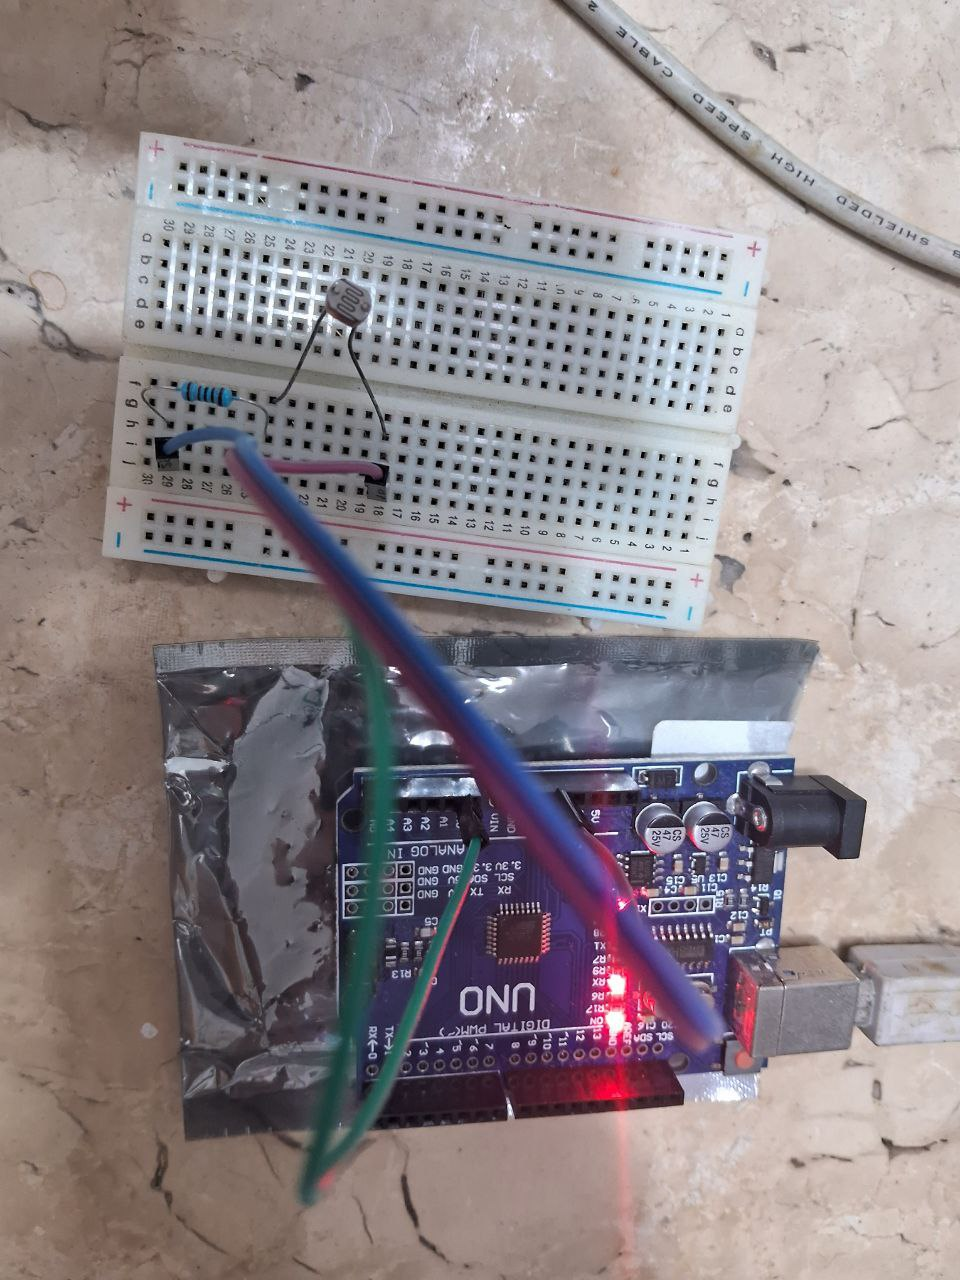
\includegraphics[width=\textwidth]{Figuras/ldr1.jpg}

            \end{figure}
        \end{column}

        \begin{column}{0.5\textwidth}
            \begin{figure}
                \centering
                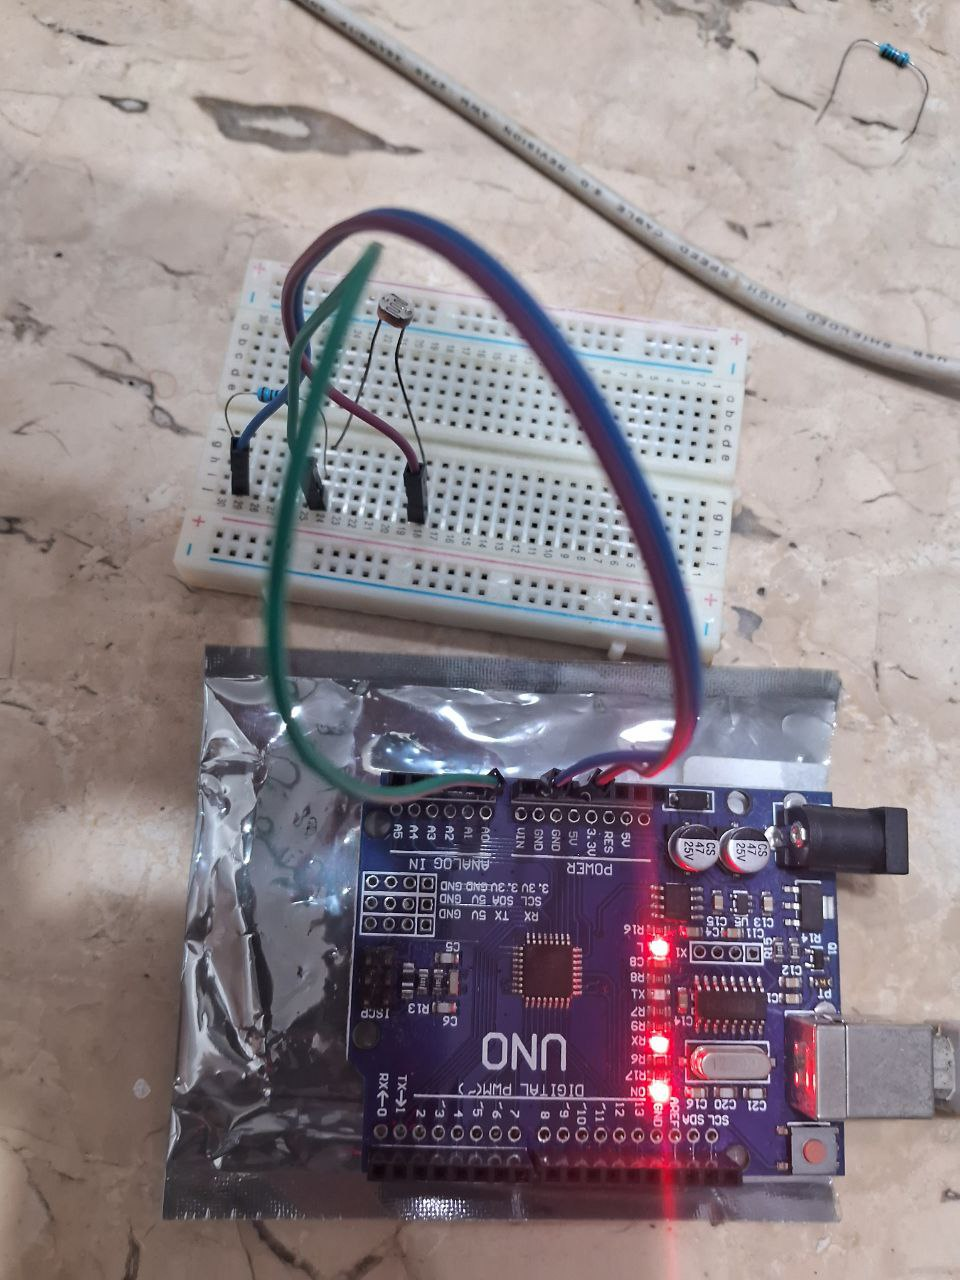
\includegraphics[width=\textwidth]{Figuras/ldr2.jpg}

            \end{figure}
        \end{column}
    \end{columns}
\end{frame}

\begin{frame}{Função \texttt{analogRead()}}
    \begin{itemize}
        \item \textbf{Descrição:} Lê o valor de um pino de entrada analógica especificado.
        \item \textbf{Conversor Analógico-Digital (ADC):}
              \begin{itemize}
                  \item O Arduino UNO possui um ADC de \textbf{10 bits}.
                  \item Mapeia tensões entre $0$ e $5\,\text{V}$ em valores inteiros entre \textbf{0 e 1023}.
              \end{itemize}
        \item \textbf{Resolução do Sistema:}
              \begin{itemize}
                  \item Cálculo: $\frac{5\,\text{V}}{1024 \text{ unidades}} \approx 0,0049\,\text{V}$ ($4,9\,\text{mV}$) por unidade.
              \end{itemize}
    \end{itemize}



    \begin{block}{Observações Técnicas}
        \begin{itemize}
            \item \textbf{analogReference():} Altera a faixa de tensão de entrada.
            \item \textbf{analogReadResolution():} Permite alterar a resolução em placas que suportam mais de 10 bits.
        \end{itemize}
    \end{block}

    \href{https://docs.arduino.cc/language-reference/en/functions/analog-io/analogRead/}{Link da API de referência}
\end{frame}

\begin{frame}{Lógica de Medição Indireta}
    \begin{itemize}
        \item \textbf{Uma cadeia:}
              \begin{enumerate}
                  \item \textbf{Fenômeno Físico:} Intensidade de luz varia.
                  \item \textbf{Efeito Analógico:} A resistência do LDR muda, alterando a \textbf{tensão ($V$)} no divisor de tensão.
                  \item \textbf{Processamento:} O microcontrolador lê essa tensão contínua.
                  \item \textbf{Interpretação:} O software associa o valor digital à condição de "escuro".
              \end{enumerate}
    \end{itemize}



    \vspace{0.3cm}
    \centering
    Nesse caso medimos a luz indiretamente através da tradução de grandezas elétricas
\end{frame}

\begin{frame}{Sistemas de Numeração Digital}
    \begin{itemize}
        \item \textbf{Panorama Geral:} Na tecnologia digital, utilizamos diferentes bases numéricas para finalidades específicas.
        \item \textbf{Os Três Pilares:}
              \begin{itemize}
                  \item \textbf{Decimal (Base 10):} Sistema utilizado por humanos no dia a dia.
                  \item \textbf{Binário (Base 2):} Linguagem nativa dos sistemas digitais (níveis lógicos).
                  \item \textbf{Hexadecimal (Base 16):} Forma compacta que facilita para humanos a leitura e escrita de grandes sequências binárias.
              \end{itemize}
    \end{itemize}



    \begin{block}{Princípio Unificado}
        Embora as bases sejam diferentes, todos esses sistemas funcionam sob a mesma lógica posicional. Entender a fundo o sistema decimal é a chave para dominar os demais.
    \end{block}
\end{frame}

\begin{frame}{Sistema Decimal (Base 10)}
    \begin{itemize}
        \item \textbf{Símbolos:} Composto por 10 dígitos: $\{0, 1, 2, 3, 4, 5, 6, 7, 8, 9\}$.
        \item \textbf{Origem:} Evoluiu do uso dos dez dedos das mãos para contagem
        \item \textit{dígito} vem do latim \textit{digitus}, "dedo".
        \item \textbf{Sistema Posicional:} O valor de um dígito depende da sua posição no número.
    \end{itemize}

    \begin{exampleblock}{Exemplo: Número 453}
        \centering
        \begin{tabular}{c c c}
            \textbf{4}        & \textbf{5}       & \textbf{3}        \\
            Centenas ($10^2$) & Dezenas ($10^1$) & Unidades ($10^0$) \\
        \end{tabular}
    \end{exampleblock}

    \begin{itemize}
        \item \textbf{MSD (Most Significant Digit):} O dígito de maior peso (neste caso, o \textbf{4}).
        \item \textbf{LSD (Least Significant Digit):} O dígito de menor peso (neste caso, o \textbf{3}).
    \end{itemize}

\end{frame}

\begin{frame}{Valor Posicional e Potências de 10}
    \begin{itemize}
        \item \textbf{A Vírgula Decimal:} Atua como o separador entre a parte \textbf{inteira} (potências positivas) e a parte \textbf{fracionária} (potências negativas).
        \item \textbf{Estrutura de Pesos:} Cada posição possui um peso que é uma potência de 10 ($10^n$).
    \end{itemize}

    \begin{exampleblock}{Decomposição do número 2745,214}
        $$ (2 \times 10^3) + (7 \times 10^2) + (4 \times 10^1) + (5 \times 10^0) + (2 \times 10^{-1}) + (1 \times 10^{-2}) + (4 \times 10^{-3}) $$
    \end{exampleblock}

    \begin{itemize}
        \item \textbf{Regra Geral:} Qualquer número é a soma dos produtos de cada dígito pelo seu valor posicional.
    \end{itemize}


\end{frame}

\begin{frame}{Exemplo}
    \begin{center}
        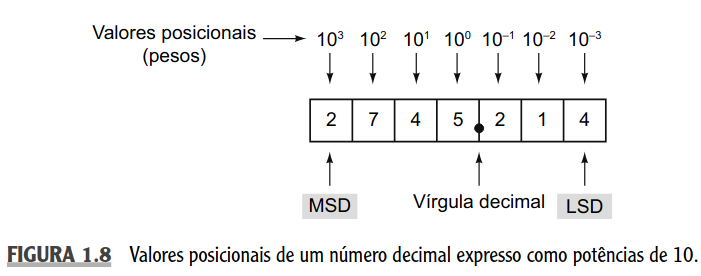
\includegraphics[width=\textwidth]{Figuras/MSDLSD.png}

    \end{center}


\end{frame}
\title{Aula 2 - Sistemas de Numeração Digital}



\begin{frame}
    \titlepage
\end{frame}



\begin{frame}{Sistemas de Numeração Digital}
    \begin{itemize}
        \item \textbf{Panorama Geral:} Na tecnologia digital, utilizamos diferentes bases numéricas para finalidades específicas.
        \item \textbf{Bases mais usadas:}
              \begin{itemize}
                  \item \textbf{Decimal (Base 10)}
                  \item \textbf{Binário (Base 2)}
                  \item \textbf{Octal (Base 8)}
                  \item \textbf{Hexadecimal (Base 16)}
              \end{itemize}
    \end{itemize}

\end{frame}

\begin{frame}{Sistema Decimal (Base 10)}
    \begin{itemize}
        \item \textbf{Símbolos:} Composto por 10 dígitos: $\{0, 1, 2, 3, 4, 5, 6, 7, 8, 9\}$.
        \item \textbf{Origem:} Evoluiu do uso dos dez dedos das mãos para contagem
        \item \textit{dígito} vem do latim \textit{digitus}, "dedo".
        \item \textbf{Sistema Posicional:} O valor de um dígito depende da sua posição no número.
    \end{itemize}
\end{frame}


\begin{frame}{Contagem decimal}
    \begin{center}
        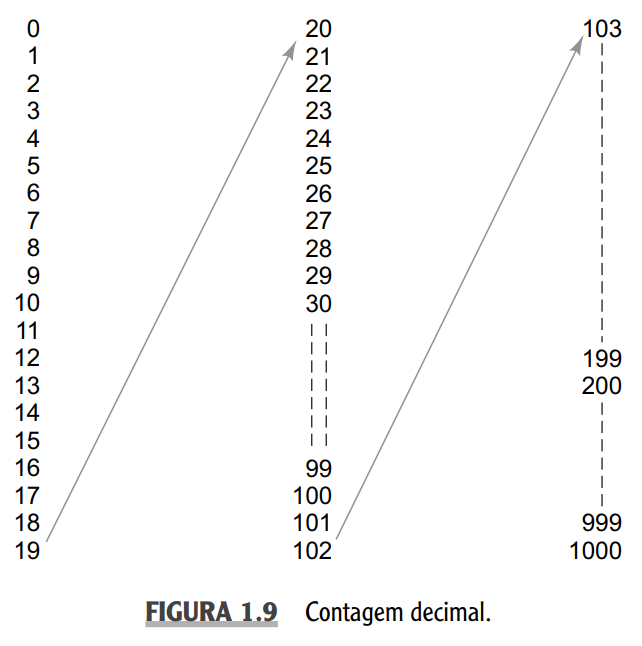
\includegraphics[width=0.7\textwidth]{Figuras/contagem-decimal.png}

    \end{center}


\end{frame}

\begin{frame}{Sistema Decimal (Base 10)}
    \begin{exampleblock}{Exemplo: Número 453}
        \centering
        \begin{tabular}{c c c}
            \textbf{4}        & \textbf{5}       & \textbf{3}        \\
            Centenas ($10^2$) & Dezenas ($10^1$) & Unidades ($10^0$) \\
        \end{tabular}
    \end{exampleblock}

    \begin{itemize}
        \item \textbf{MSD (Most Significant Digit):} O dígito de maior peso (neste caso, o \textbf{4}).
        \item \textbf{LSD (Least Significant Digit):} O dígito de menor peso (neste caso, o \textbf{3}).
    \end{itemize}

\end{frame}

\begin{frame}{Representação Formal do Sistema Decimal}
    \begin{itemize}
        \item \textbf{Estrutura Genérica:} Qualquer número decimal pode ser escrito como uma sequência de dígitos $d$ em relação à vírgula:
              $$d_n d_{n-1} \dots d_1 d_0 , d_{-1} d_{-2} \dots d_{-k}$$
    \end{itemize}

    \begin{block}{Expansão Polinomial}
        O valor real é a soma de cada dígito multiplicado pelo peso de sua posição:
        $$Valor = \sum_{i=-k}^{n} d_i \times 10^i$$
    \end{block}

    \begin{itemize}
        \item \textbf{Componentes:}
              \begin{itemize}
                  \item $d_i$: O algarismo na posição $i$ (de 0 a 9).
                  \item $10^i$: O peso (base elevada à posição).
                  \item $n$ e $k$: Número de dígitos inteiros e fracionários, respectivamente.
              \end{itemize}
    \end{itemize}

    \vspace{0.2cm}
    \centering
    \textit{Essa mesma lógica será aplicada ao sistema binário, apenas trocando a base 10 por 2.}
\end{frame}

\begin{frame}{Formalização da Notação Posicional}
    \begin{itemize}
        \item \textbf{Definição:} A posição do dígito determina a potência da base pela qual ele será multiplicado.
        \item Assim, representamos infinitos valores com um conjunto finito de símbolos.
    \end{itemize}

    \begin{block}{Formalizando}
        Para definir um sistema posicional, precisamos de:
        \begin{enumerate}
            \item \textbf{Uma Base ($B$):} O número de símbolos distintos.
            \item \textbf{Conjunto de Símbolos:} Valores inteiros de $0$ até $B-1$.
        \end{enumerate}
    \end{block}



\end{frame}



\begin{frame}{Representação Genérica em Base $B$}
    Com a base ($B$) e o conjunto de símbolos definidos, temos:

    \begin{itemize}
        \item \textbf{Sequência de dígitos:} $s = b_i$, para $i \in -k \dots n$.
        \item \textbf{Cálculo do Valor:}
    \end{itemize}

    \begin{block}{Fórmula Geral}
        $$ \text{Valor} = \sum_{i=-k}^{n} b_i B^i $$
    \end{block}

    \begin{itemize}
        \item \textbf{Expansão da Soma:}
              {\small
                  $$ b_n B^n + b_{n-1} B^{n-1} + \dots + b_0 B^0 + b_{-1} B^{-1} + \dots + b_{-k} B^{-k} $$
              }
        \item \textbf{Convenção de Escrita:} A posição menos significativa fica sempre à direita:
              $$ b_n b_{n-1} \dots b_1 b_0 , b_{-1} \dots b_{-k+1} b_{-k} $$
    \end{itemize}
\end{frame}

\begin{frame}{Exemplo de Decomposição: Inteiros (Base 10)}
    Considere a sequência \textbf{347} na base 10. Aplicando a fórmula da soma de produtos pelo peso da posição:

    \begin{itemize}
        \item \textbf{Decomposição:}
    \end{itemize}

    $$ 3 \times 10^2 + 4 \times 10^1 + 7 \times 10^0 $$


    $$ 3 \times 100 + 4 \times 10 + 7 \times 1 = 300 + 40 + 7 $$

    \begin{itemize}
        \item \textbf{Resultado:}
    \end{itemize}

    $$ 347_{10} $$


\end{frame}

\begin{frame}{Exemplo de Decomposição: Fracionários (Base 10)}
    Considere a sequência \textbf{58,25} na base 10. Note o uso de potências negativas para os dígitos após a vírgula:

    \begin{itemize}
        \item \textbf{Decomposição:}
    \end{itemize}

    $$ 5 \times 10^1 + 8 \times 10^0 + 2 \times 10^{-1} + 5 \times 10^{-2} $$



    $$ 50 + 8 + \frac{2}{10} + \frac{5}{100} = 50 + 8 + 0,2 + 0,05 $$

    \begin{itemize}
        \item \textbf{Resultado:}
    \end{itemize}

    $$ 58,25_{10} $$
\end{frame}

\begin{frame}{Valor Posicional e Potências de 10}
    \begin{itemize}
        \item \textbf{A Vírgula Decimal:} Atua como o separador entre a parte \textbf{inteira} (potências positivas) e a parte \textbf{fracionária} (potências negativas).
        \item \textbf{Estrutura de Pesos:} Cada posição possui um peso que é uma potência de 10 ($10^n$).
    \end{itemize}

    \begin{exampleblock}{Decomposição do número 2745,214}
        $$ (2 \times 10^3) + (7 \times 10^2) + (4 \times 10^1) + (5 \times 10^0) + (2 \times 10^{-1}) + (1 \times 10^{-2}) + (4 \times 10^{-3}) $$
    \end{exampleblock}

    \begin{itemize}
        \item \textbf{Regra Geral:} Qualquer número é a soma dos produtos de cada dígito pelo seu valor posicional.
    \end{itemize}


\end{frame}

\begin{frame}{Exemplo}
    \begin{center}
        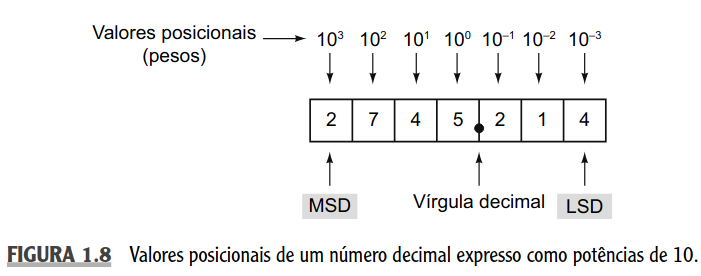
\includegraphics[width=\textwidth]{Figuras/MSDLSD.png}

    \end{center}


\end{frame}

\begin{frame}{Exercício}
    Decomponha os seguintes números decimais, considerando a notação posicional.


    \begin{enumerate}[a)]
        \item \textbf{3014}

        \item \textbf{-25,5}

        \item \textbf{10,01}


        \item \textbf{-10750}

    \end{enumerate}
\end{frame}


\begin{frame}{Exercício}
    Decomponha os seguintes números decimais, considerando a notação posicional.




    \begin{enumerate}[a)]
        \item \textbf{3014}
              \begin{itemize}
                  \item $(3 \times 10^3) + (0 \times 10^2) + (1 \times 10^1) + (4 \times 10^0)$
              \end{itemize}

        \item \textbf{-25,5}
              \begin{itemize}
                  \item $-( (2 \times 10^1) + (5 \times 10^0) + (5 \times 10^{-1}) )$
              \end{itemize}

        \item \textbf{10,01}
              \begin{itemize}
                  \item $(1 \times 10^1) + (0 \times 10^0) + (0 \times 10^{-1}) + (1 \times 10^{-2})$
              \end{itemize}

        \item \textbf{-10750}
              \begin{itemize}
                  \item $-( (1 \times 10^4) + (0 \times 10^3) + (7 \times 10^2) + (5 \times 10^1) + (0 \times 10^0) )$
              \end{itemize}
    \end{enumerate}


    \textit{Nota: O sinal é uma informação adicional à esquerda e não segue a convenção de posição/expoente.}


\end{frame}


\title{Aula 2 - Utilizando outras bases}



\begin{frame}
    \titlepage
\end{frame}


\begin{frame}{Comparativo de Bases e Símbolos}
    \begin{itemize}
        \item Seguindo a regra do intervalo $[0, B-1]$, temos os seguintes conjuntos:
    \end{itemize}

    \begin{table}[]
        \centering
        \begin{tabular}{|l|c|l|c|}
            \hline
            \textbf{Sistema} & \textbf{Base ($B$)} & \textbf{Símbolos Disponíveis} & \textbf{Intervalo} \\ \hline
            Binário          & 2                   & 0, 1                          & $0$ a $B-1$        \\ \hline
            Octal            & 8                   & 0, 1, 2, 3, 4, 5, 6, 7        & $0$ a $B-1$        \\ \hline
            Decimal          & 10                  & 0, 1, 2, 3, 4, 5, 6, 7, 8, 9  & $0$ a $B-1$        \\ \hline
            Hexadecimal      & 16                  & 0-9, A, B, C, D, E, F         & $0$ a $B-1$        \\ \hline
        \end{tabular}
    \end{table}

    \begin{block}{Convenção para Bases Maiores ($B > 10$)}
        Como não existem algarismos únicos para valores acima de 9, usamos letras:
        \centering
        \textbf{A}=10, \textbf{B}=11, \textbf{C}=12, \textbf{D}=13, \textbf{E}=14, \textbf{F}=15
    \end{block}
\end{frame}

\begin{frame}{Bases de Numeração: Base 10 (Decimal)}
    \begin{itemize}
        \item \textbf{Uso:} Base com a qual estamos familiarizados e interagimos como usuários.
        \item \textbf{Notação:}
              \begin{itemize}
                  \item Indicada pelo índice $_{10}$.
                  \item \textbf{Padrão (Default):} Se não houver indicação de base, assume-se que o número é decimal.
              \end{itemize}
    \end{itemize}

    \begin{exampleblock}{Exemplos}
        \centering
        $345$ \quad ou \quad $345_{10}$
    \end{exampleblock}
\end{frame}

\begin{frame}{Bases de Numeração: Base 2 (Binária)}
    \begin{itemize}
        \item \textbf{Uso:} Linguagem nativa dos circuitos digitais.
        \item \textbf{Notação Acadêmica:} Indicada pelo índice $_2$.
        \item \textbf{Em Programação:} Precedida pelos caracteres \texttt{0B} ou \texttt{0b}.
    \end{itemize}

    \begin{exampleblock}{Exemplos}
        \centering
        $10111_2$ \quad ou \quad \texttt{0b10111}
    \end{exampleblock}


\end{frame}

\begin{frame}{Bases de Numeração: Base 8 (Octal)}
    \begin{itemize}
        \item \textbf{Notação Acadêmica:} Indicada pelo índice $_8$.
        \item \textbf{Em Programação:}
              \begin{itemize}
                  \item Precedida por \texttt{0O} ou \texttt{0o}.
                  \item Em algumas linguagens (como C antigo), precedida apenas por \texttt{0}.
              \end{itemize}
    \end{itemize}

    \begin{exampleblock}{Exemplos}
        \centering
        $107_8$ \quad ou \quad \texttt{0o107} \quad ou \quad \texttt{0107}
    \end{exampleblock}
\end{frame}



\begin{frame}{Bases de Numeração: Base 16 (Hexadecimal)}
    \begin{itemize}
        \item \textbf{Uso:} Representação compacta de binários.
        \item \textbf{Notação Acadêmica:} Indicada pelo índice $_{16}$.
        \item \textbf{Em Programação:} Precedida pelos caracteres \texttt{0X} ou \texttt{0x}.
    \end{itemize}

    \begin{exampleblock}{Exemplos}
        \centering
        $1C7_{16}$ \quad ou \quad \texttt{0x1C7}
    \end{exampleblock}

    \begin{alertblock}{Lembrete}
        Utiliza dígitos de 0 a 9 e as letras de A a F (para representar de 10 a 15).
    \end{alertblock}
\end{frame}

\begin{frame}{Valores de 0 a 15 nas bases 2, 8, 10 e 16}
    \begin{table}[h]
        \begin{center}
            \begin{tabular}{|c|c|c|c|}
                \hline
                10 & 2    & 8  & 16 \\
                \hline
                0  & 0    & 0  & 0  \\
                1  & 1    & 1  & 1  \\
                2  & 10   & 2  & 2  \\
                3  & 11   & 3  & 3  \\
                4  & 100  & 4  & 4  \\
                5  & 101  & 5  & 5  \\
                6  & 110  & 6  & 6  \\
                7  & 111  & 7  & 7  \\
                8  & 1000 & 10 & 8  \\
                9  & 1001 & 11 & 9  \\
                10 & 1010 & 12 & A  \\
                11 & 1011 & 13 & B  \\
                12 & 1100 & 14 & C  \\
                13 & 1101 & 15 & D  \\
                14 & 1110 & 16 & E  \\
                15 & 1111 & 17 & F  \\
                \hline
            \end{tabular}
        \end{center}
    \end{table}
\end{frame}

\begin{frame}{Exercício: Contagem em Múltiplas Bases}

    Escreva os números de 0 a 20 nas seguintes bases:

    2, 5, 8, 10, 11 e 16.

    \vspace{0.3cm}
    \begin{alertblock}{Dicas!}
        \begin{itemize}
            \item Na \textbf{Base 5}, o número após o $4$ é o $10_5$.
            \item Na \textbf{Base 11}, o número $10$ é representado pela letra $A$.
        \end{itemize}
    \end{alertblock}
\end{frame}

\begin{frame}{Gabarito: Contagem de 0 a 20 em Diferentes Bases}
    \centering
    \resizebox{0.7\textwidth}{!}{
        \begin{tabular}{|c|c|c|c|c|c|}
            \hline
            \textbf{Base 10} & \textbf{Base 2} & \textbf{Base 5} & \textbf{Base 8} & \textbf{Base 11} & \textbf{Base 16} \\ \hline
            0                & 0               & 0               & 0               & 0                & 0                \\ \hline
            1                & 1               & 1               & 1               & 1                & 1                \\ \hline
            2                & 10              & 2               & 2               & 2                & 2                \\ \hline
            3                & 11              & 3               & 3               & 3                & 3                \\ \hline
            4                & 100             & 4               & 4               & 4                & 4                \\ \hline
            5                & 101             & \textbf{10}     & 5               & 5                & 5                \\ \hline
            6                & 110             & 11              & 6               & 6                & 6                \\ \hline
            7                & 111             & 12              & 7               & 7                & 7                \\ \hline
            8                & 1000            & 13              & \textbf{10}     & 8                & 8                \\ \hline
            9                & 1001            & 14              & 11              & 9                & 9                \\ \hline
            10               & 1010            & 20              & 12              & \textbf{A}       & A                \\ \hline
            11               & 1011            & 21              & 13              & \textbf{10}      & B                \\ \hline
            12               & 1100            & 22              & 14              & 11               & C                \\ \hline
            13               & 1101            & 23              & 15              & 12               & D                \\ \hline
            14               & 1110            & 24              & 16              & 13               & E                \\ \hline
            15               & 1111            & 30              & 17              & 14               & F                \\ \hline
            16               & 10000           & 31              & 20              & 15               & \textbf{10}      \\ \hline
            17               & 10001           & 32              & 21              & 16               & 11               \\ \hline
            18               & 10010           & 33              & 22              & 17               & 12               \\ \hline
            19               & 10011           & 34              & 23              & 18               & 13               \\ \hline
            20               & 10100           & 40              & 24              & 19               & 14               \\ \hline
        \end{tabular}
    }
\end{frame}


\title{Aula 3 - Conversão de bases}



\begin{frame}
    \titlepage
\end{frame}


\begin{frame}{Conversão de uma base qualquer para base 10}
    Para converter um número de qualquer base $B$ para a base $10$, aplicamos a definição da notação posicional, realizando os cálculos na base 10:

    \begin{block}{Fórmula Única}
        $$ \text{Valor}_{10} = \sum_{i=-k}^{n} b_i B^i $$
    \end{block}

    \begin{itemize}
        \item \textbf{Passo a passo:}
              \begin{enumerate}
                  \item Identifique o peso (potência de $B$) de cada posição.
                  \item Multiplique o dígito pelo seu peso.
                  \item Some todos os resultados.
              \end{enumerate}
    \end{itemize}
\end{frame}

\begin{frame}{Exemplos - Conversão de Binário e Octal para a base 10}
    \begin{itemize}
        \item \textbf{Converver de Binário ($B=2$) para decimal:} $10100,1_2$
              {\small
              $$ (1 \times 2^4) + (0 \times 2^3) + (1 \times 2^2) + (0 \times 2^1) + (0 \times 2^0) + (1 \times 2^{-1}) $$
              $$ 16 + 0 + 4 + 0 + 0 + 0,5 = \mathbf{20,5_{10}} $$
              }

              \vspace{0.4cm}

        \item \textbf{Converver de Octal ($B=8$) para decimal:} $253_8$
              {\small
                      $$ (2 \times 8^2) + (5 \times 8^1) + (3 \times 8^0) $$
                      $$ (2 \times 64) + (5 \times 8) + (3 \times 1) $$
                      $$ 128 + 40 + 3 = \mathbf{171_{10}} $$
                  }
    \end{itemize}
\end{frame}

\begin{frame}{Exemplos de Conversão: Hexadecimal}
    \begin{itemize}
        \item \textbf{Converver de Hexadecimal ($B=16$) para decimal:} $C3_{16}$
    \end{itemize}

    \begin{exampleblock}{Lembrete Importante}
        No sistema hexadecimal, letras devem ser substituídas pelos seus valores decimais antes do cálculo: \textbf{C = 12}.
    \end{exampleblock}

    $$ (C \times 16^1) + (3 \times 16^0) $$
    $$ (12 \times 16) + (3 \times 1) $$
    $$ 192 + 3 = \mathbf{195_{10}} $$
\end{frame}

\begin{frame}{Exercícios: Conversão para Base 10}
    Converta os seguintes números para a base 10, demonstrando a decomposição posicional:

    \begin{enumerate}[a)]
        \item $11011,01_2$
        \item $702_8$
        \item $BF_{16}$
    \end{enumerate}

    \vspace{0.5cm}
    \begin{center}
        \textit{Dica: Comece identificando os expoentes da base a partir da vírgula (para a esquerda $0, 1, 2...$ e para a direita $-1, -2...$).}
    \end{center}
\end{frame}

\begin{frame}{Resposta $11011,01_2$ para decimal}
    \begin{center}
        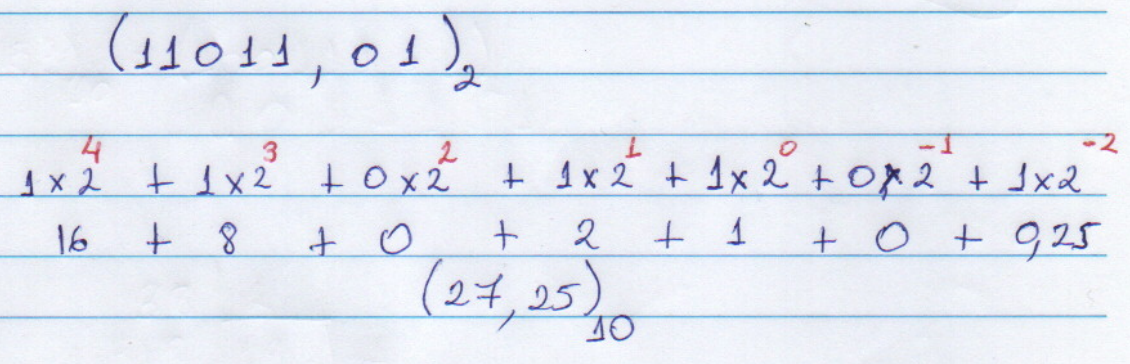
\includegraphics[width=0.9\textwidth]{Figuras/11011-01-to-dec.png}

    \end{center}

    $11011,01_2 = 27,25_{10}$
\end{frame}

\begin{frame}{Resposta $702_8$ para decimal}
    \begin{center}
        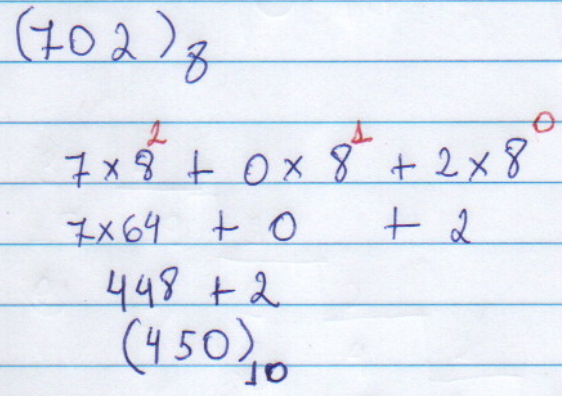
\includegraphics[width=0.9\textwidth]{Figuras/702-to-dec.png}

    \end{center}

    $702_8 = 450_{10}$
\end{frame}

\begin{frame}{Resposta $BF_{16}$ para decimal}
    \begin{center}
        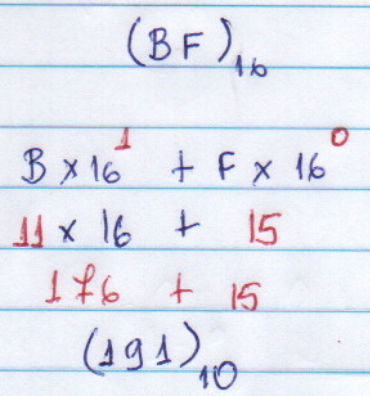
\includegraphics[width=0.5\textwidth]{Figuras/BF-to-dec.png}

    \end{center}

    $BF_{16} = 191_{10}$
\end{frame}

\begin{frame}{Conversão de Decimal para uma base qualquer}
    \begin{itemize}
        \item \textbf{O Método:} Divisões Sucessivas pela base de destino.
        \item \textbf{Propriedade 1:} O resto da primeira divisão é o dígito de menor peso ($b_0$).
        \item \textbf{Propriedade 2:} Ao dividir o quociente sucessivamente, obtemos os dígitos seguintes ($b_1, b_2, \dots$).
        \item \textbf{Encerramento:} O processo termina quando o \textbf{quociente é zero}.
    \end{itemize}

    \begin{block}{Formando o número}
        O resultado é formado pela leitura dos \textbf{restos} na ordem \textbf{inversa} (do último para o primeiro).
    \end{block}
\end{frame}

\begin{frame}{Exemplo Passo a Passo: $9_{10}$ para Binário}
    Vamos converter o número 9 para a base 2:
    \begin{enumerate}
        \item $9 \div 2 = 4$ com \textbf{resto 1} $\rightarrow (b_0)$
        \item $4 \div 2 = 2$ com \textbf{resto 0} $\rightarrow (b_1)$
        \item $2 \div 2 = 1$ com \textbf{resto 0} $\rightarrow (b_2)$
        \item $1 \div 2 = 0$ com \textbf{resto 1} $\rightarrow (b_3)$
    \end{enumerate}

    \begin{exampleblock}{Resultado}
        Lendo os restos do último para o primeiro: $\mathbf{1001_2}$
        $$ 9 = 1 \times 2^3 + 0 \times 2^2 + 0 \times 2^1 + 1 \times 2^0 $$
    \end{exampleblock}
\end{frame}

\begin{frame}{Exemplo do método das divisões sucessivas}
    \begin{center}
        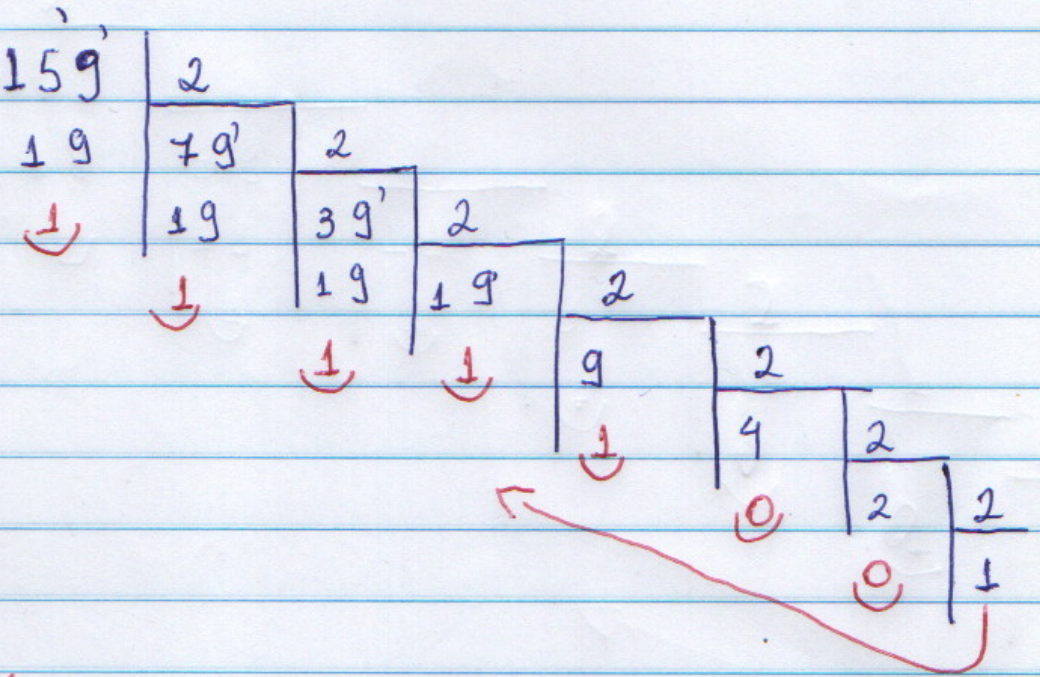
\includegraphics[width=0.7\textwidth]{Figuras/159-to-bin.png}

    \end{center}

    $159_{10} = 10011111_{2}$
\end{frame}

\begin{frame}{Exemplo do método das divisões sucessivas}
    \begin{center}
        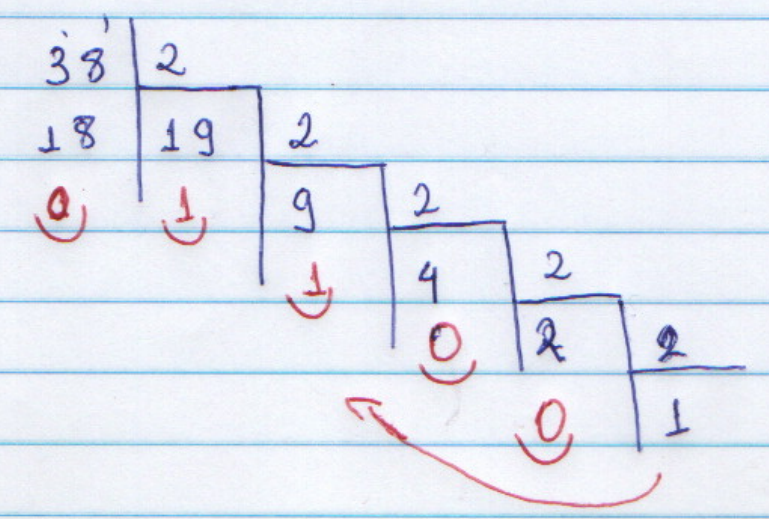
\includegraphics[width=0.7\textwidth]{Figuras/38-to-bin.png}

    \end{center}

    $38_{10} = 100110_{2}$
\end{frame}



\begin{frame}{Conversão: $352_{10}$ para Octal}
    Utilizar uma tabela ajuda a organizar o processo para números maiores:

    \begin{table}[]
        \centering
        \begin{tabular}{|c|c|c|c|c|}
            \hline
            \textbf{Índice} & \textbf{Dividendo} & \textbf{Divisor} & \textbf{Quociente} & \textbf{Resto} \\ \hline
            0               & 352                & 8                & 44                 & \textbf{0}     \\ \hline
            1               & 44                 & 8                & 5                  & \textbf{4}     \\ \hline
            2               & 5                  & 8                & 0                  & \textbf{5}     \\ \hline
        \end{tabular}
    \end{table}

    \begin{itemize}
        \item Lendo os restos de baixo para cima: \textbf{5}, \textbf{4}, \textbf{0}.
        \item \textbf{Resultado:} $352_{10} = 540_8$
    \end{itemize}
\end{frame}

\begin{frame}{Exemplo do método das divisões sucessivas}
    \begin{center}
        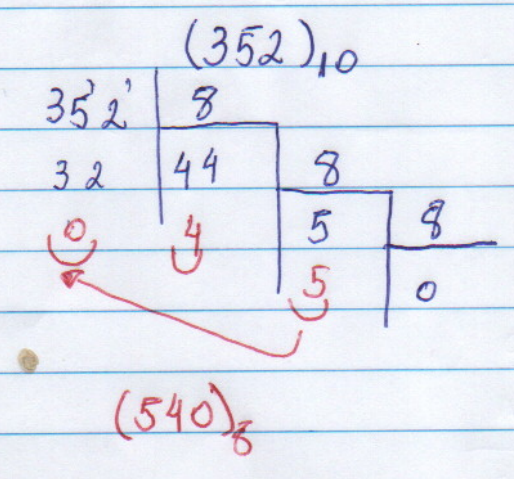
\includegraphics[width=0.7\textwidth]{Figuras/352-to-oct.png}

    \end{center}

    $352_{10} = 540_8$
\end{frame}

\begin{frame}{Conversão de $352_{10}$ para Binário}

    \centering
    \resizebox{\textwidth}{!}{
        \begin{tabular}{|c|c|c|c|c|}
            \hline
            \textbf{Índice} & \textbf{Dividendo} & \textbf{Divisor} & \textbf{Quociente} & \textbf{Resto} \\ \hline
            0               & 352                & 2                & 176                & \textbf{0}     \\ \hline
            1               & 176                & 2                & 88                 & \textbf{0}     \\ \hline
            2               & 88                 & 2                & 44                 & \textbf{0}     \\ \hline
            3               & 44                 & 2                & 22                 & \textbf{0}     \\ \hline
            4               & 22                 & 2                & 11                 & \textbf{0}     \\ \hline
            5               & 11                 & 2                & 5                  & \textbf{1}     \\ \hline
            6               & 5                  & 2                & 2                  & \textbf{1}     \\ \hline
            7               & 2                  & 2                & 1                  & \textbf{0}     \\ \hline
            8               & 1                  & 2                & 0                  & \textbf{1}     \\ \hline
        \end{tabular}
    }
    \\

    Lendo os restos do índice 8 ao 0:
    $101100000_2$


\end{frame}

\begin{frame}{Exercício}

    Escreva sua \textbf{idade} e o \textbf{ano atual} nas seguintes bases, utilizando o método das divisões sucessivas:

    \begin{enumerate}[a)]
        \item Base 11
        \item Base 2
        \item Base 8
        \item Base 16
    \end{enumerate}


\end{frame}

\begin{frame}{Casos especiais onde uma base é potência da outra}



    \begin{itemize}
        \item Para converter de uma base para outra qualquer, sempre é possível
              converter para a base 10 e em seguida da
              base 10 para a base final.

        \item No entanto, em alguns casos (quando uma base é uma potência da outra)
              pode-se evitar esse trabalho.

        \item As técnicas para as bases mais usadas em computação (2, 8 e 16) são exemplificadas a seguir.
    \end{itemize}




\end{frame}

\begin{frame}{Conversão de números em base 8 para base 2}


    \begin{itemize}
        \item A base octal (8) é uma potência da base binária (2): $8 = 2^3$.
        \item Isso permite uma conversão direta e simplificada.
        \item Vamos desenvolver o raciocínio por trás do método.
    \end{itemize}

\end{frame}

\begin{frame}{Passo 1: Expansão posicional - Reescrevendo na base 2}


    Considere o número $253_8$:

    \begin{align*}
        253_8 & = 3 \times 8^0 + 5 \times 8^1 + 2 \times 8^2                                    \\
              & = 3 \times (2^3)^0 + 5 \times (2^3)^1 + 2 \times (2^3)^2                        \\
              & = 3 \times 2^{(3 \times 0)} + 5 \times 2^{3 \times 1} + 2 \times 2^{3 \times 2} \\
              & = 3 \times 2^0 + 5 \times 2^{3} + 2 \times 2^{6}
    \end{align*}

\end{frame}

\begin{frame}{Passo 2: Tentativa inicial}


    \begin{itemize}
        \item Temos os coeficientes $3$, $5$ e $2$ multiplicando potências de $2$.
        \item Seria tentador escrever $2005003_2$, colocando cada dígito em sua posição (0, 3 e 6).

        \item \textbf{Problema:} $2$, $5$ e $3$ \textbf{não são dígitos válidos} na base binária (que só aceita $0$ e $1$).
        \item Precisamos traduzir esses valores ($3$, $5$ e $2$) para sua representação binária.
    \end{itemize}


    \textbf{ATENÇÃO}, nessa hora tome cuidado com mistura de bases

\end{frame}

\begin{frame}{Passo 3: Decomposição dos coeficientes}
    \emph{Transformando $3$, $5$ e $2$ em somas de potências de 2}

    \begin{align*}
        3 & = 1 + 2 =  1 \times 2^0 + 1 \times 2^1 \\
        5 & = 1 + 4 =  1 \times 2^0 + 1 \times 2^2 \\
        2 & = 0 + 2 =  1 \times 2^1
    \end{align*}

\end{frame}

\begin{frame}{Passo 4: Substituição e desenvolvimento}


    \begin{align*}
        253_8 & =  3 \times 2^0 + 5 \times 2^{3} + 2 \times 2^{6}     \\
              & = (1 \times 2^0 + 1 \times 2^1) \times 2^0 \; +       \\
              & \quad (1 \times 2^0 + 1 \times 2^2) \times 2^{3} \; + \\
              & \quad (1 \times 2^1) \times 2^{6}
    \end{align*}

\end{frame}

\begin{frame}{Passo 5: Simplificação}


    Distribuindo e somando os expoentes:

    \begin{align*}
        253_8 & = (1 \times 2^{0}) + (1 \times 2^{1}) \; +     \\
              & \quad (1 \times 2^{3}) + (1 \times 2^{5}) \; + \\
              & \quad (1 \times 2^{7})                         \\[0.5cm]
              & = 2^0 + 2^1 + 2^3 + 2^5 + 2^7
    \end{align*}

\end{frame}

\begin{frame}{Passo 6: O número binário resultante}


    A soma das potências de 2 nos dá a representação binária final:

    \[
        2^0 + 2^1 + 2^3 + 2^5 + 2^7 = 10101011_2
    \]

    Ou seja, $253_8 = 10101011_2$.

\end{frame}

\begin{frame}{Passo-a-passo feito a mão}
    \begin{center}
        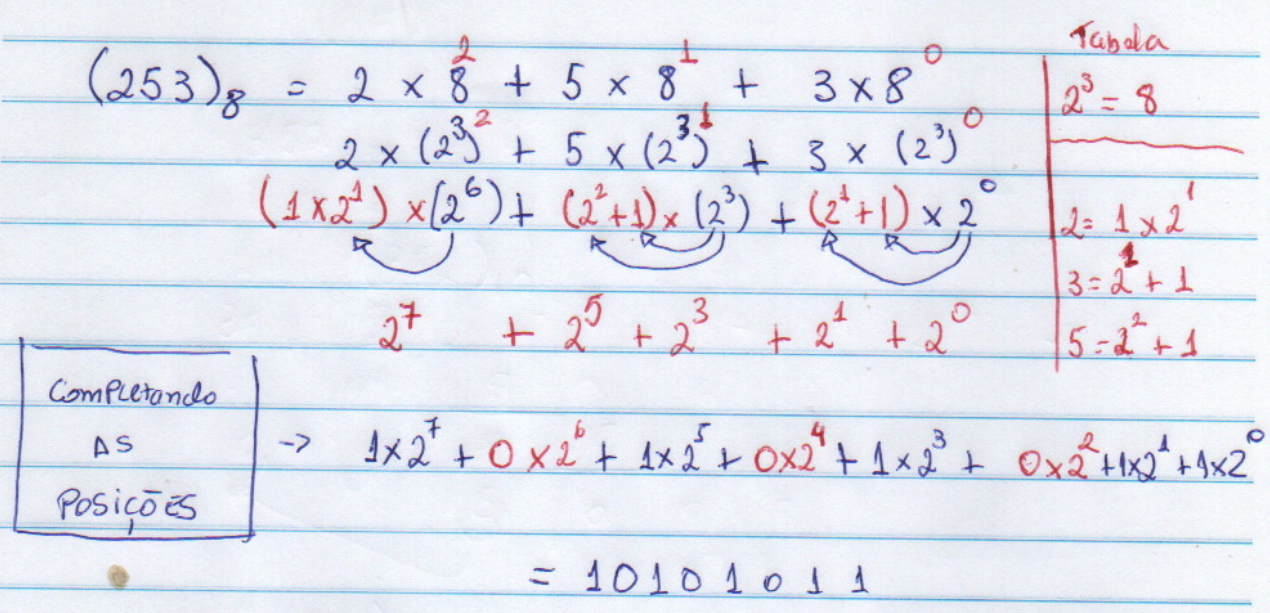
\includegraphics[width=\textwidth]{Figuras/conversao-direta-metodo.png}

    \end{center}


\end{frame}

\begin{frame}{Consequência do resultado anterior}


    O desenvolvimento anterior justifica o método que vamos realmente aplicar:

    \begin{block}{Como fazer?}
        Cada símbolo da representação \textbf{octal} deve ser expandido em sua representação com \textbf{3 bits}.
    \end{block}

    \begin{itemize}
        \item Devem-se usar \textbf{zeros à esquerda} para completar os 3 bits em símbolos menores que 4 ($100_2$).
    \end{itemize}

    \vspace{0.3cm}
    \textbf{Exemplo:} Sabendo que $2_8 = 010_2$, $5_8 = 101_2$ e $3_8 = 011_2$:

    \begin{itemize}
        \item $253_8 = \underbrace{010}_{2} \text{ concat. com } \underbrace{101}_{5} \text{ concat. com } \underbrace{011}_{3}$
    \end{itemize}
\end{frame}

\begin{frame}{Exemplo fazendo a concatenação}


    Ao realizar a junção dos grupos de 3 bits, temos:

    \begin{exampleblock}{Conversão Final}
        $$253_8 = 010101011_2$$
    \end{exampleblock}

    \vspace{0.5cm}
    \begin{itemize}
        \item $253_8 = 10101011_2$
    \end{itemize}

    \begin{alertblock}{Observação Importantíssima}
        O zero mais à esquerda ($010...$) pode ser \textbf{omitido}, uma vez que a concatenação foi finalizada e ele não altera o valor do número.
    \end{alertblock}
\end{frame}



\begin{frame}{Tabela de Conversão: Octal $\rightarrow$ Binário}
    \begin{itemize}
        \item Como $8 = 2^3$, cada dígito octal é \textbf{3 bits} na representação binária.
        \item Tabela de Substituição dígito octal por binário de 3 bits.
    \end{itemize}

    \begin{table}[]
        \centering
        \Large
        \begin{tabular}{|c|c|}
            \hline
            \textbf{Digito Octal} & \textbf{3 dígitos em Binário} \\
            \hline
            $0_8$                 & $000_2$                       \\ \hline
            $1_8$                 & $001_2$                       \\ \hline
            $2_8$                 & $010_2$                       \\ \hline
            $3_8$                 & $011_2$                       \\ \hline
            $4_8$                 & $100_2$                       \\ \hline
            $5_8$                 & $101_2$                       \\ \hline
            $6_8$                 & $110_2$                       \\ \hline
            $7_8$                 & $111_2$                       \\ \hline
        \end{tabular}
    \end{table}

\end{frame}

\begin{frame}{Exemplo: Conversão Binário $\rightarrow$ Octal}
    Convertendo $11100_2$ para octal - Método Prático
    \begin{itemize}
        \item Para converter binário em octal, agrupamos os bits de \textbf{3 em 3} a partir da direita.
        \item $11100_2 = \underbrace{11}_{\text{grupo 1}} \underbrace{100}_{\text{grupo 2}}$
        \item Completamos com zero à esquerda se necessário: $011\ 100$
        \item Cada grupo de 3 bits é convertido independentemente:
    \end{itemize}

    \begin{table}[h]
        \centering
        \begin{tabular}{c|c|c}
            \textbf{Grupo}     & \textbf{Bits} & \textbf{Octal} \\
            \hline
            Grupo 1 (esquerda) & $011_2$       & $3_8$          \\
            Grupo 2 (direita)  & $100_2$       & $4_8$          \\
        \end{tabular}
    \end{table}

    \begin{itemize}
        \item Concatenando os dígitos octais: $3$ e $4$
        \item Portanto: $\boxed{11100_2 = 34_8}$
    \end{itemize}

\end{frame}

\begin{frame}{Exemplo: Conversão Binário $\rightarrow$ Octal (Visualização)}
    %-------------------Figure---------------------
    \begin{figure}[h]
        \centering
        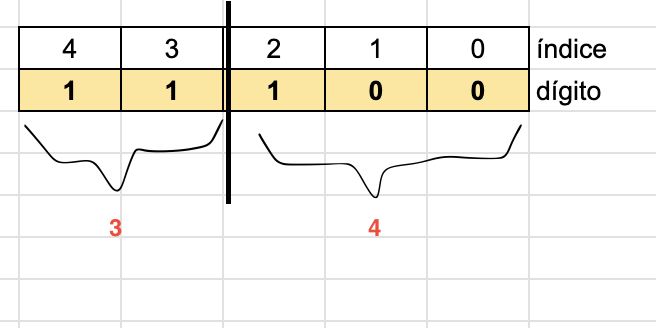
\includegraphics[width=0.6\textwidth]{Figuras/agrupamento_de2_para8.png}
        \label{fig-agrupamento2-8}
    \end{figure}
    %-------------------Figure---------------------


    \begin{align*}
        11100_2 & = 1\times2^4 + 1\times2^3 + 1\times2^2 + 0\times2^1 + 0\times2^0 \\
                & = 2^4 + 2^3 + 2^2                                                \\
                & = (2^1 + 2^0) \times 2^3 + 2^2                                   \\
                & = (2 + 1) \times 8 + 4                                           \\
                & = 3 \times 8 + 4                                                 \\
                & = 3 \times 8^1 + 4 \times 8^0                                    \\
                & = 34_8
    \end{align*}



\end{frame}

\begin{frame}{Conversão: Base 16 para Base 2}

    Como $16 = 2^4$, cada símbolo da representação hexadecimal corresponde a um grupo de \textbf{4 bits}.



    \textbf{Procedimento:}
    \begin{itemize}
        \item Cada dígito hexadecimal deve ser expandido em sua representação binária de 4 bits.
        \item \textbf{Atenção:} Deve-se usar zeros à esquerda para completar os 4 bits em valores menores que $8$ (ex: $1_{16} \rightarrow 0001_2$).
    \end{itemize}
\end{frame}

\begin{frame}{Exemplo Detalhado: $1C_{16}$}
    Vamos decompor o número $1C_{16}$ utilizando potências de 2:

    \begin{itemize}
        \item $1C_{16} = C \times 16^0 + 1 \times 16^1$
        \item $1C_{16} = 12 \times 16^0 + 1 \times 16^1$
        \item $1C_{16} = 12 \times (2^4)^0 + 1 \times (2^4)^1$
        \item $1C_{16} = 12 \times 2^0 + 1 \times 2^4$
    \end{itemize}

    Sabendo que $C_{16} = 12_{10} = 1100_2$ (ou $2^3 + 2^2$), substituímos:

    \begin{itemize}
        \item $1C_{16} = (2^3 + 2^2) \times 2^0 + 1 \times 2^4$
        \item $1C_{16} = 2^3 + 2^2 + 2^4$
        \item $1C_{16} = 11100_2$
    \end{itemize}
\end{frame}

\begin{frame}{Tabela de Conversão: Hexadecimal $\rightarrow$ Binário}
    \begin{itemize}
        \item Como $16 = 2^4$, cada dígito hexadecimal corresponde a \textbf{4 bits} na representação binária.
        \item Substituímos cada símbolo pelo seu equivalente binário de 4 dígitos.
    \end{itemize}

    \begin{table}[]
        \centering
        \small
        \begin{tabular}{|c|c||c|c|}
            \hline
            \textbf{Hex} & \textbf{4 bits Binário} & \textbf{Hex} & \textbf{4 bits Binário} \\ \hline
            $0_{16}$     & $0000_2$                & $8_{16}$     & $1000_2$                \\ \hline
            $1_{16}$     & $0001_2$                & $9_{16}$     & $1001_2$                \\ \hline
            $2_{16}$     & $0010_2$                & $A_{16}$     & $1010_2$                \\ \hline
            $3_{16}$     & $0011_2$                & $B_{16}$     & $1011_2$                \\ \hline
            $4_{16}$     & $0100_2$                & $C_{16}$     & $1100_2$                \\ \hline
            $5_{16}$     & $0101_2$                & $D_{16}$     & $1101_2$                \\ \hline
            $6_{16}$     & $0110_2$                & $E_{16}$     & $1110_2$                \\ \hline
            $7_{16}$     & $0111_2$                & $F_{16}$     & $1111_2$                \\ \hline
        \end{tabular}
    \end{table}
\end{frame}

\begin{frame}{Método Simplificado (Mapeamento Direto)}
    A forma mais rápida é a concatenação de grupos de 4 bits:

    \begin{table}
        \centering
        \begin{tabular}{|c|c|}
            \hline
            \textbf{Hexadecimal} & \textbf{Binário (4 bits)} \\ \hline
            $1_{16}$             & $0001_2$                  \\ \hline
            $C_{16}$             & $1100_2$                  \\ \hline
        \end{tabular}
    \end{table}

    \vspace{0.3cm}
    \textbf{Resultado:}
    \begin{displaymath}
        1C_{16} = \underbrace{0001}_{1} \underbrace{1100}_{C} = 00011100_2
    \end{displaymath}

    \vspace{0.3cm}
    Removendo os zeros à esquerda:
    $$1C_{16} = 11100_2$$
\end{frame}

\begin{frame}{Exercício}
    Converta \textbf{sem passar para a base 10} os seguintes números da base 8 para a base 2:


    \begin{enumerate}[a)]
        \item $20_8$
        \item $7_8$
        \item $407_8$
        \item $2022_8$

    \end{enumerate}

    Converta \textbf{sem passar para a base 10} os seguintes números da base 16 para a base 2:
    \begin{enumerate}[a)]
        \item  $20_{16}$
        \item  $7_{16}$
        \item  $407_{16}$
        \item  $2022_{16}$
        \item  $ABCD_{16}$
    \end{enumerate}
\end{frame}

\begin{frame}{Exercício -- Gabarito}
    Converta \textbf{sem passar para a base 10} os seguintes números da base 8 para a base 2 \textcolor{red}{grupos de 3 bits}:

    \begin{enumerate}[a)]
        % \hfill empurra o texto para a direita, \textcolor{red} muda a cor
        \item $20_8$ = \textcolor{red}{$010\,000_2 = 10000_2$}
        \item $7_8$ = \textcolor{red}{$111_2$}
        \item $407_8$ = \textcolor{red}{$100\,000\,111_2$}
        \item $2022_8$ = \textcolor{red}{$010\,000\,010\,010_2 = 10000010010_2$}
    \end{enumerate}

    \vspace{0.3cm} % Espaçamento entre os blocos

    Converta \textbf{sem passar para a base 10} os seguintes números da base 16 para a base 2 \textcolor{red}{grupos de 4 bits}:
    \begin{enumerate}[a)]
        \item $20_{16}$ = \textcolor{red}{$0010\,0000_2 = 100000_2$}
        \item $7_{16}$ = \textcolor{red}{$0111_2 = 111_2$}
        \item $407_{16}$ = \textcolor{red}{$0100\,0000\,0111_2 = 10000000111_2$}
        \item $2022_{16}$ = \textcolor{red}{$0010\,0000\,0010\,0010_2 = 10000000100010_2$}
        \item $ABCD_{16}$ = \textcolor{red}{$1010\,1011\,1100\,1101_2$}
    \end{enumerate}
\end{frame}


\title{Aula 4 - Operações aritméticas em diferentes bases}



\begin{frame}
    \titlepage
\end{frame}

\begin{frame}{Aritmética em Diferentes Bases}
    \begin{itemize}
        \item O procedimento para realizar operações aritméticas em qualquer base é aplicar a \textbf{tabuada da operação} na base correspondente.
        \item Na \textbf{base 10}, fazemos isso de forma automática devido ao treinamento precoce.
        \item Em outras bases ($2, 8, 16$), como não temos isso na nossa cabeça.
    \end{itemize}

    Como fazer soma, por exemplo:
    \begin{enumerate}
        \item Trabalhamos coluna por coluna (da direita para a esquerda).
        \item Realizamos a soma ou subtração.
        \item Se o valor exceder a base, ocorre o \textbf{"vai um"} .

    \end{enumerate}


\end{frame}

\begin{frame}{Adição Binária: A Tabuada de Bits}
    Para realizar a adição binária sem converter para a base 10, utilizamos a tabuada da operação. Por ser pequena, sua memorização é simples:

    \begin{table}[h]
        \centering
        \begin{tabular}{|c|c|c|c|}
            \hline
            \textbf{Operando 1} & \textbf{Operando 2} & \textbf{Soma} & \textbf{Vai um (Carry)} \\ \hline
            0                   & 0                   & 0             & 0                       \\ \hline
            0                   & 1                   & 1             & 0                       \\ \hline
            1                   & 0                   & 1             & 0                       \\ \hline
            1                   & 1                   & 0             & 1                       \\ \hline
        \end{tabular}
        \caption{Tabuada de adição de bits}
        \label{tabuada2+}
    \end{table}

    \begin{itemize}
        \item Quando há um "vai um", a próxima coluna passa a ter 3 operandos.
        \item Aplicamos a soma em etapas: $(1 + 1) + 1 = 10_2 + 1 = 11_2$ (soma 1 e vai 1).
    \end{itemize}
\end{frame}

\begin{frame}{Exemplo de Adição Binária: $11011_2 + 1001_2$}
    Somamos da direita para a esquerda, respeitando as colunas:

    \vspace{0.5cm}
    \centering
    \Large
    \begin{tabular}{r cccccc}
        \color{blue}{\footnotesize (vai um)} & \color{blue}{1} & \color{blue}{1} & \color{blue}{0} & \color{blue}{1} & \color{blue}{1} &                \\
                                             &                 & 1               & 1               & 0               & 1               & $1_2$          \\
        +                                    &                 &                 & 1               & 0               & 0               & $1_2$          \\ \cline{2-7}
                                             & \textbf{1}      & \textbf{0}      & \textbf{0}      & \textbf{1}      & \textbf{0}      & \textbf{0}$_2$ \\
    \end{tabular}

    \vspace{0.8cm}
    \flushleft
    \normalsize
    \textbf{Resultado:} $11011_2 + 1001_2 = 100100_2$

    \vspace{0.3cm}
    \small
    \textit{Nota: em binário, $1+1=10$ (fica 0 e vai 1) e $1+1+1=11$ (fica 1 e vai 1).}
\end{frame}

\begin{frame}{Exercício -- Operações na Base 2}
    Faça as seguintes operações na base 2 \textbf{sem converter} os números a serem somados para a base 10 (você pode converter depois de realizar o exercício para conferir o resultado!):

    \begin{enumerate}[a)]
        \item $1101_2 + 010_2$
        \item $1010_2 + 1010_2$
        \item $1111_2 + 1111_2$
        \item $101_2 + 1011_2$
    \end{enumerate}



\end{frame}


\begin{frame}{Exercício -- Operações na Base 2}
    \textbf{Gabarito} -  Faça as seguintes operações na base 2 \textbf{sem converter} os números a serem somados para a base 10 (você pode converter depois de realizar o exercício para conferir o resultado!):




    \begin{enumerate}[a)]
        \item $1101_2 + 0010_2 = 1111_2$
        \item $1010_2 + 1010_2 = 10100_2$
        \item $1111_2 + 1111_2 = 11110_2$
        \item $0101_2 + 1011_2 = 10000_2$
    \end{enumerate}

\end{frame}
\begin{frame}{Adição Octal e Hexadecimal}


    \begin{exampleblock}{Exemplo: $172_8 + 30_8$}
        \centering
        \Large
        \begin{tabular}{r ccc}
            \color{blue}{\footnotesize (carry)} & \color{blue}{1} &            &                \\
                                                & 1               & 7          & $2_8$          \\
            +                                   &                 & 3          & $0_8$          \\ \cline{2-4}
                                                & \textbf{2}      & \textbf{2} & \textbf{2$_8$} \\
        \end{tabular}
    \end{exampleblock}

    \small
    \textbf{Raciocínio por coluna:}
    \begin{itemize}
        \item \textbf{Col. 0:} $2+0 = 2_8$.
        \item \textbf{Col. 1:} $7+3 = 10_{10}$. Como $10 = (1 \times 8) + 2$, temos \textbf{$12_8$}. Fica $2$ e \textbf{vai $1$}.
        \item \textbf{Col. 2:} $1$ (carry) $+ 1 = 2_8$.
    \end{itemize}
\end{frame}

\begin{frame}{Exemplo de Adição Hexadecimal: $5D2_{16} + 5A_{16}$}
    \centering
    \begin{tabular}{r ccc}
        \color{blue}{\footnotesize (carry)} & \color{blue}{1} &            &                   \\
                                            & 5               & D          & $2_{16}$          \\
        +                                   &                 & 5          & $A_{16}$          \\ \cline{2-4}
                                            & \textbf{6}      & \textbf{2} & \textbf{C$_{16}$} \\
    \end{tabular}

    \vspace{0.4cm}
    \flushleft
    \textbf{Detalhamento do raciocínio:}
    \begin{description}
        \item[Coluna 0:] $2_{16} + A_{16} = 2 + 10 = 12_{10}$. Convertendo para hexa: \textbf{$C_{16}$}.
        \item[Coluna 1:] $D_{16} + 5_{16} = 13 + 5 = 18_{10}$. \\
              Como $18 = (1 \times 16) + 2$, temos \textbf{$12_{16}$}. Fica $2$ e \textbf{vai $1$}.
        \item[Coluna 2:] $1$ (carry) $+ 5 = 6_{16}$.
    \end{description}

    \vspace{0.4cm}
    \textbf{Resultado:} $5D2_{16} + 5A_{16} = 62C_{16}$
\end{frame}

\begin{frame}{Exercícios: Adição em Bases 8 e 16}
    Realize as seguintes operações \textbf{sem converter os números para a base 10}:

    \begin{block}{Base 8 (Octal)}
        \begin{enumerate}[a)]
            \item $5_8 + 6_8$
            \item $27_8 + 11_8$
            \item $256_8 + 525_8$
        \end{enumerate}
    \end{block}

    \vspace{0.5cm}

    \begin{block}{Base 16 (Hexadecimal)}
        \begin{enumerate}[a)]
            \item $503C_{16} + 8_{16}$
            \item $503C_{16} + 64_{16}$
        \end{enumerate}
    \end{block}

    \vspace{0.3cm}
    \small
    \textit{Dica: Some coluna por coluna e lembre-se do "vai um" sempre que o valor atingir ou superar a base.}
\end{frame}

\begin{frame}{Gabarito: Adição em Bases 8 e 16}
    \textbf{Resultados na Base 8:}
    \begin{enumerate}[a)]
        \item $5_8 + 6_8$ = \textcolor{red}{$13_8$}
        \item $27_8 + 11_8$ =  \textcolor{red}{$40_8$}
        \item $256_8 + 525_8$ = \textcolor{red}{$1003_8$}
    \end{enumerate}

    \vspace{0.6cm}

    \textbf{Resultados na Base 16:}
    \begin{enumerate}[a)]
        \item $503C_{16} + 8_{16}$ = \textcolor{red}{$5044_{16}$}
        \item $503C_{16} + 64_{16}$ = \textcolor{red}{$50A0_{16}$}
    \end{enumerate}
\end{frame}

\begin{frame}{Subtração em Diferentes Bases}
    \begin{itemize}
        \item \textbf{Subtração Simples:} Quando o dígito do minuendo (cima) é maior ou igual ao do subtraendo (baixo).
        \item \textbf{Subtração com Empréstimo:} Quando o dígito de cima é menor que o de baixo, precisamos "pedir emprestado" à coluna da esquerda.
    \end{itemize}

    \begin{block}{A Regra do Empréstimo (Borrow)}
        \begin{enumerate}
            \item O dígito da esquerda (posição $i+1$) perde \textbf{1}.
            \item O dígito atual (posição $i$) ganha o \textbf{valor da base} ($2, 8$ ou $16$).
        \end{enumerate}
    \end{block}

    \begin{table}[h]
        \centering
        \small
        \begin{tabular}{|c|c|c|c|}
            \hline
            \textbf{Minuendo} & \textbf{Subtraendo} & \textbf{Diferença} & \textbf{Vem um (Borrow)} \\ \hline
            0                 & 0                   & 0                  & 0                        \\ \hline
            0                 & 1                   & \textbf{1}         & \textbf{1 (Empréstimo)}  \\ \hline
            1                 & 0                   & 1                  & 0                        \\ \hline
            1                 & 1                   & 0                  & 0                        \\ \hline
        \end{tabular}
        \caption{Tabuada de subtração de bits}
    \end{table}
\end{frame}

\begin{frame}{Exemplo 1: Subtração Binária Simples}
    Neste caso, todos os bits de cima são maiores ou iguais aos de baixo:

    \vspace{0.8cm}
    \centering
    \Large
    \begin{tabular}{r ccccc}
          & 1          & 1          & 0          & 1          & $1_2$          \\
        - &            & 1          & 0          & 0          & $1_2$          \\ \cline{2-6}
          & \textbf{1} & \textbf{0} & \textbf{0} & \textbf{1} & \textbf{0$_2$} \\
    \end{tabular}

    \vspace{0.8cm}
    \flushleft
    \normalsize
    \textbf{Resultado:} $11011_2 - 1001_2 = 10010_2$
\end{frame}

\begin{frame}{Exemplo 2: Subtração com Empréstimo}
    Quando temos $0 - 1$, pedimos emprestado à esquerda. O $1$ vira $0$ e a coluna atual ganha $10_2$ (que vale $2_{10}$).

    \vspace{0.5cm}
    \centering
    \Large
    \begin{tabular}{r cccccl}
        \color{red}{\footnotesize (emprestado)} & \color{red}{-1} & \color{red}{-1} & \color{red}{+10} &            &                & \\
                                                & 1               & 1               & 0                & 1          & $1_2$          & \\
        -                                       &                 & 1               & 1                & 0          & $1_2$          & \\ \cline{2-6}
                                                & \textbf{0}      & \textbf{1}      & \textbf{1}       & \textbf{1} & \textbf{0$_2$} & \\
    \end{tabular}

    \vspace{0.5cm}
    \flushleft
    \small
    \textbf{Raciocínio:}
    \begin{itemize}
        \item \textbf{Col. 2:} $0 - 1$ não dá. Pede emprestado: o $1$ da Col. 3 vira $0$. A Col. 2 vira $10_2$. $10_2 - 1 = 1$.
        \item \textbf{Col. 3:} Era $1$, virou $0$. $0 - 1$ não dá. Pede à Col. 4. O $1$ da Col. 4 vira $0$. A Col. 3 vira $10_2$. $10_2 - 1 = 1$.
    \end{itemize}
    \normalsize
    \textbf{Resultado:} $11011_2 - 1101_2 = 1110_2$
\end{frame}

\begin{frame}{Exercícios: Subtração Binária}
    Realize as seguintes operações \textbf{sem converter os números para a base 10}.


    \begin{enumerate}[a)]
        \item $1101_2 - 100_2$
        \item $1010_2 - 101_2$
        \item $1000_2 - 111_2$
        \item $10011_2 - 101_2$
    \end{enumerate}


    \vspace{0.5cm}


\end{frame}
\begin{frame}{Gabarito: Subtração Binária}


    \begin{enumerate}[a)]
        \item $1101_2 - 0100_2 =$  \textcolor{red}{$1001_2$}


        \item $1010_2 - 0101_2 =$  \textcolor{red}{$101_2$}


        \item $1000_2 - 0111_2 =$  \textcolor{red}{$1_2$}


        \item $10011_2 - 00101_2 =$  \textcolor{red}{$1110_2$}

    \end{enumerate}

    \vspace{0.3cm}
    \centering
    \normalsize
    \textbf{Dica:} Para conferir, some o resultado com o subtraendo!
\end{frame}

\begin{frame}{Subtração Octal}
    Diferente da base 10, o empréstimo aqui vale \textbf{8}.

    \begin{columns}
        \begin{column}{0.45\textwidth}
            \begin{exampleblock}{Sem Empréstimo}
                \centering
                \begin{tabular}{r ccc}
                      & 1          & 7          & $2_8$          \\
                    - &            & 3          & $0_8$          \\ \cline{2-4}
                      & \textbf{1} & \textbf{4} & \textbf{2$_8$} \\
                \end{tabular}
            \end{exampleblock}
            \small \textit{Sem empréstimo, a sequência de símbolos é idêntica à base 10.}
        \end{column}

        \begin{column}{0.52\textwidth}
            \begin{exampleblock}{Com Empréstimo}
                \centering
                \begin{tabular}{r ccc}
                    \color{red}{\footnotesize (emprestado)} & \color{red}{-1} & \color{red}{+$10_8$} &                \\
                                                            & 1               & 2                    & $2_8$          \\
                    -                                       &                 & 7                    & $0_8$          \\ \cline{2-4}
                                                            & \textbf{0}      & \textbf{3}           & \textbf{2$_8$} \\
                \end{tabular}
            \end{exampleblock}
            \footnotesize
            \textbf{Raciocínio Col. 1:} \\
            $2_8 < 7_8 \rightarrow$ pede emprestado. \\
            $(2 + 8)_{10} = 10_{10}$. \\
            $10 - 7 = 3$. Resultado: \textbf{$3_8$}.
        \end{column}
    \end{columns}
\end{frame}

\begin{frame}{Subtração Hexadecimal: Exemplo $5D2_{16} - 5A_{16}$}
    \centering
    \Large
    \begin{tabular}{r ccc}
        \color{red}{\footnotesize (emprestado)} &            & \color{red}{-1} & \color{red}{+$10_{16}$} \\
                                                & 5          & D               & $2_{16}$                \\
        -                                       &            & 5               & $A_{16}$                \\ \cline{2-4}
                                                & \textbf{5} & \textbf{7}      & \textbf{8$_{16}$}       \\
    \end{tabular}

    \vspace{0.4cm}
    \flushleft
    \normalsize \textbf{Detalhamento:}
    \begin{itemize}
        \item \textbf{Col. 0:} $2 < A (10)$. Pede emprestado: $(2 + 16)_{10} = 18_{10}$. \\
              $18 - 10 = 8$. Resultado: \textbf{$8_{16}$}.
        \item \textbf{Col. 1:} O $D (13)$ emprestou 1, virou $C (12)$. \\
              $12 - 5 = 7$. Resultado: \textbf{$7_{16}$}.
        \item \textbf{Col. 2:} $5 - 0 = 5$.
    \end{itemize}
\end{frame}

\begin{frame}{Exercícios: Subtração Octal e Hexadecimal}
    Realize as operações diretamente na base indicada:

    \begin{block}{Base 8 (Octal)}
        \begin{enumerate}[a)]
            \item $254_8 - 123_8$
            \item $56_8 - 37_8$
        \end{enumerate}
    \end{block}

    \begin{block}{Base 16 (Hexadecimal)}
        \begin{enumerate}[a)]
            \item $503C_{16} - 40_{16}$
            \item $50EA_{16} - 503C_{16}$
        \end{enumerate}
    \end{block}

    \vspace{0.3cm}
    \centering
    \small \textit{Dica: Converta o símbolo para decimal apenas para fazer a conta da coluna, depois volte para a base original.}
\end{frame}

\begin{frame}{Gabarito: Subtração Octal e Hexadecimal}
    \textbf{Respostas Base 8:}
    \begin{enumerate}[a)]
        \item $254_8 - 123_8 =$  \textcolor{red}{$131_8$}
        \item $56_8 - 37_8  $=\textcolor{red}{$17_8$}
    \end{enumerate}

    \vspace{0.8cm}

    \textbf{Respostas Base 16:}
    \begin{enumerate}[a)]
        \item $503C_{16} - 40_{16} $= \textcolor{red}{$4FFC_{16}$}
        \item $50EA_{16} - 503C_{16} $  = \textcolor{red}{$AE_{16}$}
    \end{enumerate}

    \vspace{0.3cm}
    \footnotesize \textit{*No item (a) de Hexa, o 0 da posição 503C precisou pedir emprestado ao 5, tornando-se 15 ($F$) após passar o empréstimo adiante.}
\end{frame}

\begin{frame}{Multiplicação em Qualquer Base}
    \begin{itemize}
        \item O processo segue a mesma lógica da base 10: multiplicamos cada dígito do segundo operando por todos os dígitos do primeiro.
        \item Cada nova linha de produto parcial é deslocada uma posição à esquerda.
        \item O resultado final é a \textbf{soma} de todos os produtos parciais.
    \end{itemize}

    \begin{block}{Multiplicação Binária}
        No mundo binário, a operação é simplificada:
        \begin{itemize}
            \item Se o multiplicador é \textbf{1}: Copiamos o primeiro operando.
            \item Se o multiplicador é \textbf{0}: A linha será composta apenas por zeros.
        \end{itemize}
    \end{block}
\end{frame}

\begin{frame}{Multiplicação Binária: A Regra}
    A multiplicação binária é baseada em uma tabuada muito simples. Na prática, multiplicamos o primeiro operando bit a bit pelos dígitos do segundo operando.



    \begin{tabular}{|c|c|c|}
        \hline
        \textbf{Primeiro número} & \textbf{Segundo número} & \textbf{Produto} \\ \hline
        0                        & 0                       & 0                \\ \hline
        0                        & 1                       & 0                \\ \hline
        1                        & 0                       & 0                \\ \hline
        1                        & 1                       & 1                \\ \hline
    \end{tabular}



    O que observar:
    \begin{itemize}
        \item Multiplicar por \textbf{1} é apenas repetir o número.
        \item Multiplicar por \textbf{0} resulta em zero.
        \item Lembre-se de deslocar cada linha de produto parcial à esquerda.
    \end{itemize}

\end{frame}

\begin{frame}{Exemplo de Multiplicação: $11011_2 \times 1001_2$}


    \begin{figure}[h]
        \centering
        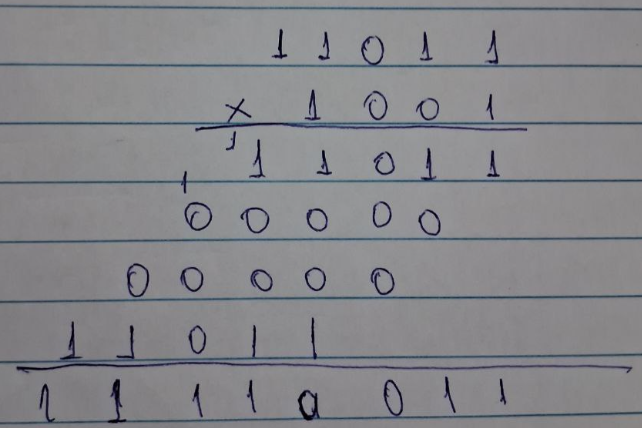
\includegraphics[width=0.7\textwidth]{Figuras/multiplicacao.png}

    \end{figure}

    \vspace{0.8cm}
    \flushleft
    \normalsize
    \textbf{Dica:} Após gerar as linhas de produto, aplique a regra da \textbf{soma binária} com atenção aos "vai um" (carries) gerados.
\end{frame}

\begin{frame}{Multiplicação Octal e Hexadecimal}
    \begin{itemize}
        \item O processo exige converter os produtos parciais para decimal e depois reconvertê-los para a base original.
        \item \textbf{Importante:} O "vai um" (carry) aqui pode ser qualquer valor, dependendo de quantas vezes a base cabe no resultado do produto.
    \end{itemize}

    \begin{exampleblock}{Exemplo Octal: $172_8 \times 30_8$}
        \centering
        \begin{tabular}{r ccccl}
                       & 1          & 7          & 2          & $_8$          &              \\
            $\times$   &            & 3          & 0          & $_8$          &              \\ \cline{2-5}
                       & 0          & 0          & 0          &               & ($\times 0$) \\
            + 5        & 5          & 6          &            &               & ($\times 3$) \\ \cline{2-5}
            \textbf{5} & \textbf{5} & \textbf{6} & \textbf{0} & \textbf{$_8$} &              \\
        \end{tabular}
    \end{exampleblock}

    \small
    \textbf{Raciocínio ($3 \times 172_8$):}
    \begin{itemize}
        \item $3 \times 2 = 6_8$.
        \item $3 \times 7 = 21_{10} \rightarrow (2 \times 8) + 5 = 25_8$. Fica \textbf{5} e vão \textbf{2}.
        \item $3 \times 1 = 3$. Com os 2 que foram: $3 + 2 = 5_8$.
    \end{itemize}
\end{frame}

\begin{frame}{Exemplo Hexadecimal: $5D2_{16} \times 51_{16}$}
    \centering
    \Large
    \begin{tabular}{r ccccc}
                   &            & 5          & D          & 2          & $_{16}$          \\
        $\times$   &            &            & 5          & 1          & $_{16}$          \\ \cline{2-6}
                   &            & 5          & D          & 2          & (x1)             \\
        + 1        & D          & 1          & A          &            & (x5)             \\ \cline{2-6}
        \textbf{1} & \textbf{D} & \textbf{7} & \textbf{7} & \textbf{2} & \textbf{$_{16}$} \\
    \end{tabular}

    \vspace{0.4cm}
    \flushleft
    \small
    \textbf{Destaque do cálculo (x5):}
    \begin{itemize}
        \item $5 \times 2 = 10_{10} = \mathbf{A_{16}}$.
        \item $5 \times D (13) = 65_{10} \rightarrow (4 \times 16) + 1 = \mathbf{41_{16}}$. Fica \textbf{1} e vão \textbf{4}.
        \item $5 \times 5 = 25_{10}$. Com o carry: $25 + 4 = 29_{10} \rightarrow (1 \times 16) + 13 = \mathbf{1D_{16}}$.
    \end{itemize}
\end{frame}

\begin{frame}{Exercícios: Multiplicação em Bases Diversas}
    Realize as operações diretamente na base indicada:

    \begin{block}{Binário e Octal}
        \begin{enumerate}[a)]
            \item $1010_2 \times 11_2$
            \item $1100_2 \times 101_2$
            \item $123_8 \times 43_8$
        \end{enumerate}
    \end{block}

    \begin{block}{Hexadecimal}
        \begin{enumerate}[d)]
            \item $1A2_{16} \times 21_{16}$
        \end{enumerate}
    \end{block}




\end{frame}

\begin{frame}{Gabarito: Multiplicação}
    \textbf{Respostas:}
    \begin{enumerate}[a)]
        \item $1010_2 \times 11_2 = $ \textcolor{red}{$11110_2$}
        \item $1100_2 \times 101_2 = $  \textcolor{red}{$111100_2$}



        \item $123_8 \times 43_8$=
              \textcolor{red}{$5531_8$}




        \item $1A2_{16} \times 21_{16}$=
              \textcolor{red}{$35E2_{16}$}
    \end{enumerate}
\end{frame}

\begin{frame}{Divisão Binária}
    \begin{itemize}
        \item O algoritmo é idêntico ao da divisão decimal (método da chave).
        \item \textbf{Vantagem:} Cada bit do quociente só pode ser \textbf{0} ou \textbf{1}.
              \begin{itemize}
                  \item \textbf{1:} Se o dividendo parcial for maior ou igual ao divisor.
                  \item \textbf{0:} Se o dividendo parcial for menor que o divisor.
              \end{itemize}
        \item É a operação base para implementações de hardware em camadas próximas ao processador.
    \end{itemize}

    \begin{exampleblock}{Exemplo: $100100_2 \div 111_2$}
        \begin{figure}[h]
            \centering
            % Substitua pelo caminho correto da sua imagem
            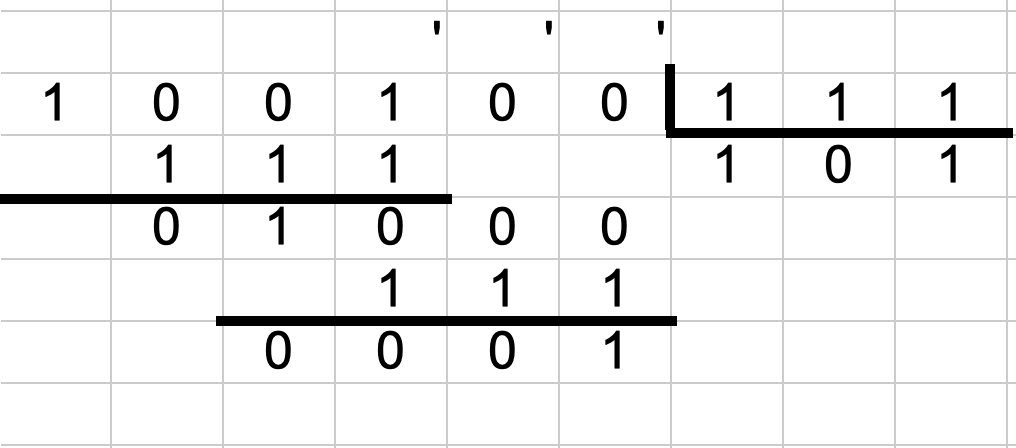
\includegraphics[width=.6\textwidth]{Figuras/divbinaria.png}
            \caption{Processo de divisão bit a bit}
            \label{fig-divbinaria}
        \end{figure}
    \end{exampleblock}
\end{frame}

\begin{frame}{Passo a Passo da Divisão: $100100_2 \div 111_2$}
    \small
    \begin{enumerate}
        \item \textbf{Busca:} Percorremos o dividendo da esquerda para a direita até encontrar um valor $\geq$ ao divisor ($111_2$).
        \item \textbf{Primeiro Bit:} Como $1001_2 \geq 111_2$, o primeiro bit do quociente é \textbf{1}.
        \item \textbf{Subtração:} $1001_2 - 111_2 = 0010_2$ (resto parcial).
        \item \textbf{Baixar Bit:} "Baixamos" o próximo $0$. O novo dividendo parcial é $100_2$.
        \item \textbf{Bit Zero:} Como $100_2 < 111_2$, o próximo bit do quociente é \textbf{0}.
        \item \textbf{Novo Bit:} Baixamos o último $0$. Agora temos $1000_2$.
        \item \textbf{Bit Um:} Como $1000_2 \geq 111_2$, o bit final do quociente é \textbf{1}.
        \item \textbf{Resto Final:} $1000_2 - 111_2 = 001_2$.
    \end{enumerate}

    \vspace{0.2cm}
    \centering
    \textbf{Resultado:} Quociente = $101_2$ | Resto = $1_2$
\end{frame}



\end{document}
